% Positron Emission tomography (includes Physics, detector basics, Event types and data types, PET ring systems and acquisition modes (2D and 3D) , Corrections, , PET WB acquisition mode and fussion -> multibed, Hybrid PET systems (PET-CT, PET-MR)) 
This section covers aspects of the main principles of \gls{pet} and serves as a brief introduction into the notions that are necessary for the description of the work carried out in this thesis. It is not an exhaustive review of the processes involved in \gls{pet} imaging. Readers can find more basics principles explained in detail in the textbooks which are frequently referenced in this chapter.

\section{Historical Perspective}
The main principles of a \Gls{pet} imaging system were developed and demonstrated with a working scanner prototype in late 1970s by Ter-Pogossian et al.~\cite{Ter-Pogossian1975} and Phelps et al.~\cite{Phelps1975}. The main concept of their prototype, which forms the basis of \gls{pet} devices, was the placement of detectors in a circular formation around the imaged object and the detection of annihilation photon pairs which serves as "Electronic" collimation. The combination of these principles makes \gls{pet} imaging superior to single photon based imaging devices still until today. 
Early systems were limited due to cost and engineering limitations to an axial coverage of a few axial planes, and were mostly used in brain imaging. Development of scanner models with higher axial \gls{fov} enabled use for imaging of other organs than the brain, where in combination with the FDG tracer (a glucose analogue tracer) quickly showed potential in detection of extra-cranial tumours~\cite{Nutt2002}.
The expanded \gls{fov} along with the capability of achieving whole-body coverage by use of shifted axial acquisitions~\cite{Dahlbom1992} (multiple axial bed positions to achieve whole-body coverage) have secured the use of \gls{pet} in oncology~\cite{Bomanji2001} and driven many more technological developments towards higher sensitivity for  improved small lesion detectability and reduction of scan time~\cite{Jones2017}.


\section{Fundamental physics of PET}

\subsection{Positron emission}
As its name suggests, \gls{pet} is an imaging method based in positron emission. Positron emission is a spontaneous process that happens as part of the β$^{+}$ decay process of radionuclides. 
Radionuclides are comprised of atoms with excess energy that decay to stable forms via routes that result to emission of radiation.
The rate at which a radionuclide undergoes decay depends on its characteristic half-life $T_{1/2}$. This is defined as the time taken for half of the nuclei of a specific radionuclide to decay. The rate of decay at any time $t$ is defined as the activity $A(t)$,measured in Becquerels (Bq), which changes over time according to
\begin{equation} \label{Decay}
A(t) = A_0 e^{-\lambda t} \ ,
\end{equation}
where $A_0$ is the activity at reference time $t_0=0$ and $\lambda$ is the decay constant, for which 
\begin{equation} \label{Decayconstant}
\lambda = \frac{ln(2)}{T_{1/2}} \ .
\end{equation}
%
Proton-rich radioisotopes decay via emission of a positron (β$^{+}$) particle and a neutrino (ν). The positron is given part of the excess radioisotope energy in the form of kinetic energy, which when emitted within a material is gradually lost from continuous interactions with other atoms of the material until the positron approaches close to a rest. During this period the positron follows a tortuous random path. The positron range can be defined for a sufficient large number of emissions as either the FWHM or mean of the distances between the emission and annihilation position. The positron range value will depend on the positrons energy spectrum and the interacting material properties. After most of its energy has been expended, the positron rapidly interacts with an electron and annihilates. This interaction results in the conversion of the two particles into two photons of 511 \si{k\electronvolt} which are emitted in almost opposite directions ($\sim$180\degree). Due to the non-zero kinetic energy during the annihilation, the excess energy sometimes results to a small acollinearity of the photon pair.
%
A list of commonly used positron emitting radioisotopes used for \gls{pet} imaging is given in table~\ref{tab:radioisotopes} along with relevant characteristics for PET imaging \cite{Conti2016}.

\begin{table}[htbp]
  \caption{Commonly used radioisotopes and their relevant characteristics for PET imaging.}
\makebox[\textwidth][c]{
    \begin{tabular}{cccc}
\toprule
  Radioisotope & Half-life & \multicolumn{1}{c}{ β$^{+}$ maximum energy (\si{M\electronvolt})} & \multicolumn{1}{c}{Mean range in water (mm)} \\
\midrule
\ce{^15O} & 2 min & 1.732 &  3.0    \\
\ce{^13N} & 10.0 min & 1.199  & 1.8  \\
\ce{^11C} & 20.4 min & 0.96 & 1.2   \\
\ce{^18F} & 110 min & 0.634 &  0.6  \\
\ce{^68Ga} & 67.8 min & 1.899 &2.9      \\
\ce{^64Cu} & 12.7 h & 0.653 &  0.7  \\
\ce{^89Zr} & 78.4 h& 0.902 & 1.3    \\
\bottomrule
\end{tabular}%
}
\label{tab:radioisotopes}%
\end{table}%

\subsection{Interactions with matter}
The range of positrons within tissue is relatively short, with the majority of positrons being annihilated within the body.
On the other hand the 511 \si{k\electronvolt} photons have less chances of interacting within the body and a large fraction of them will exit the imaged object without interacting. 

The two most probable interactions for high energy photons of 511 \si{k\electronvolt} are photoelectric absorption and Compton scattering. In photoelectric absorption the photon is completely absorbed while interacting with an atomic electron, to which it provides all of its energy. In Compton scattering the photon interacts with an atomic electron, to which it passes part of its energy. This process results in a change of direction and reduction of the energy of the original photon. Between the two processes, the Compton effect is the dominant interaction for 511 \si{k\electronvolt} photons in tissue. 
%
\begin{figure} [h!]
\centering
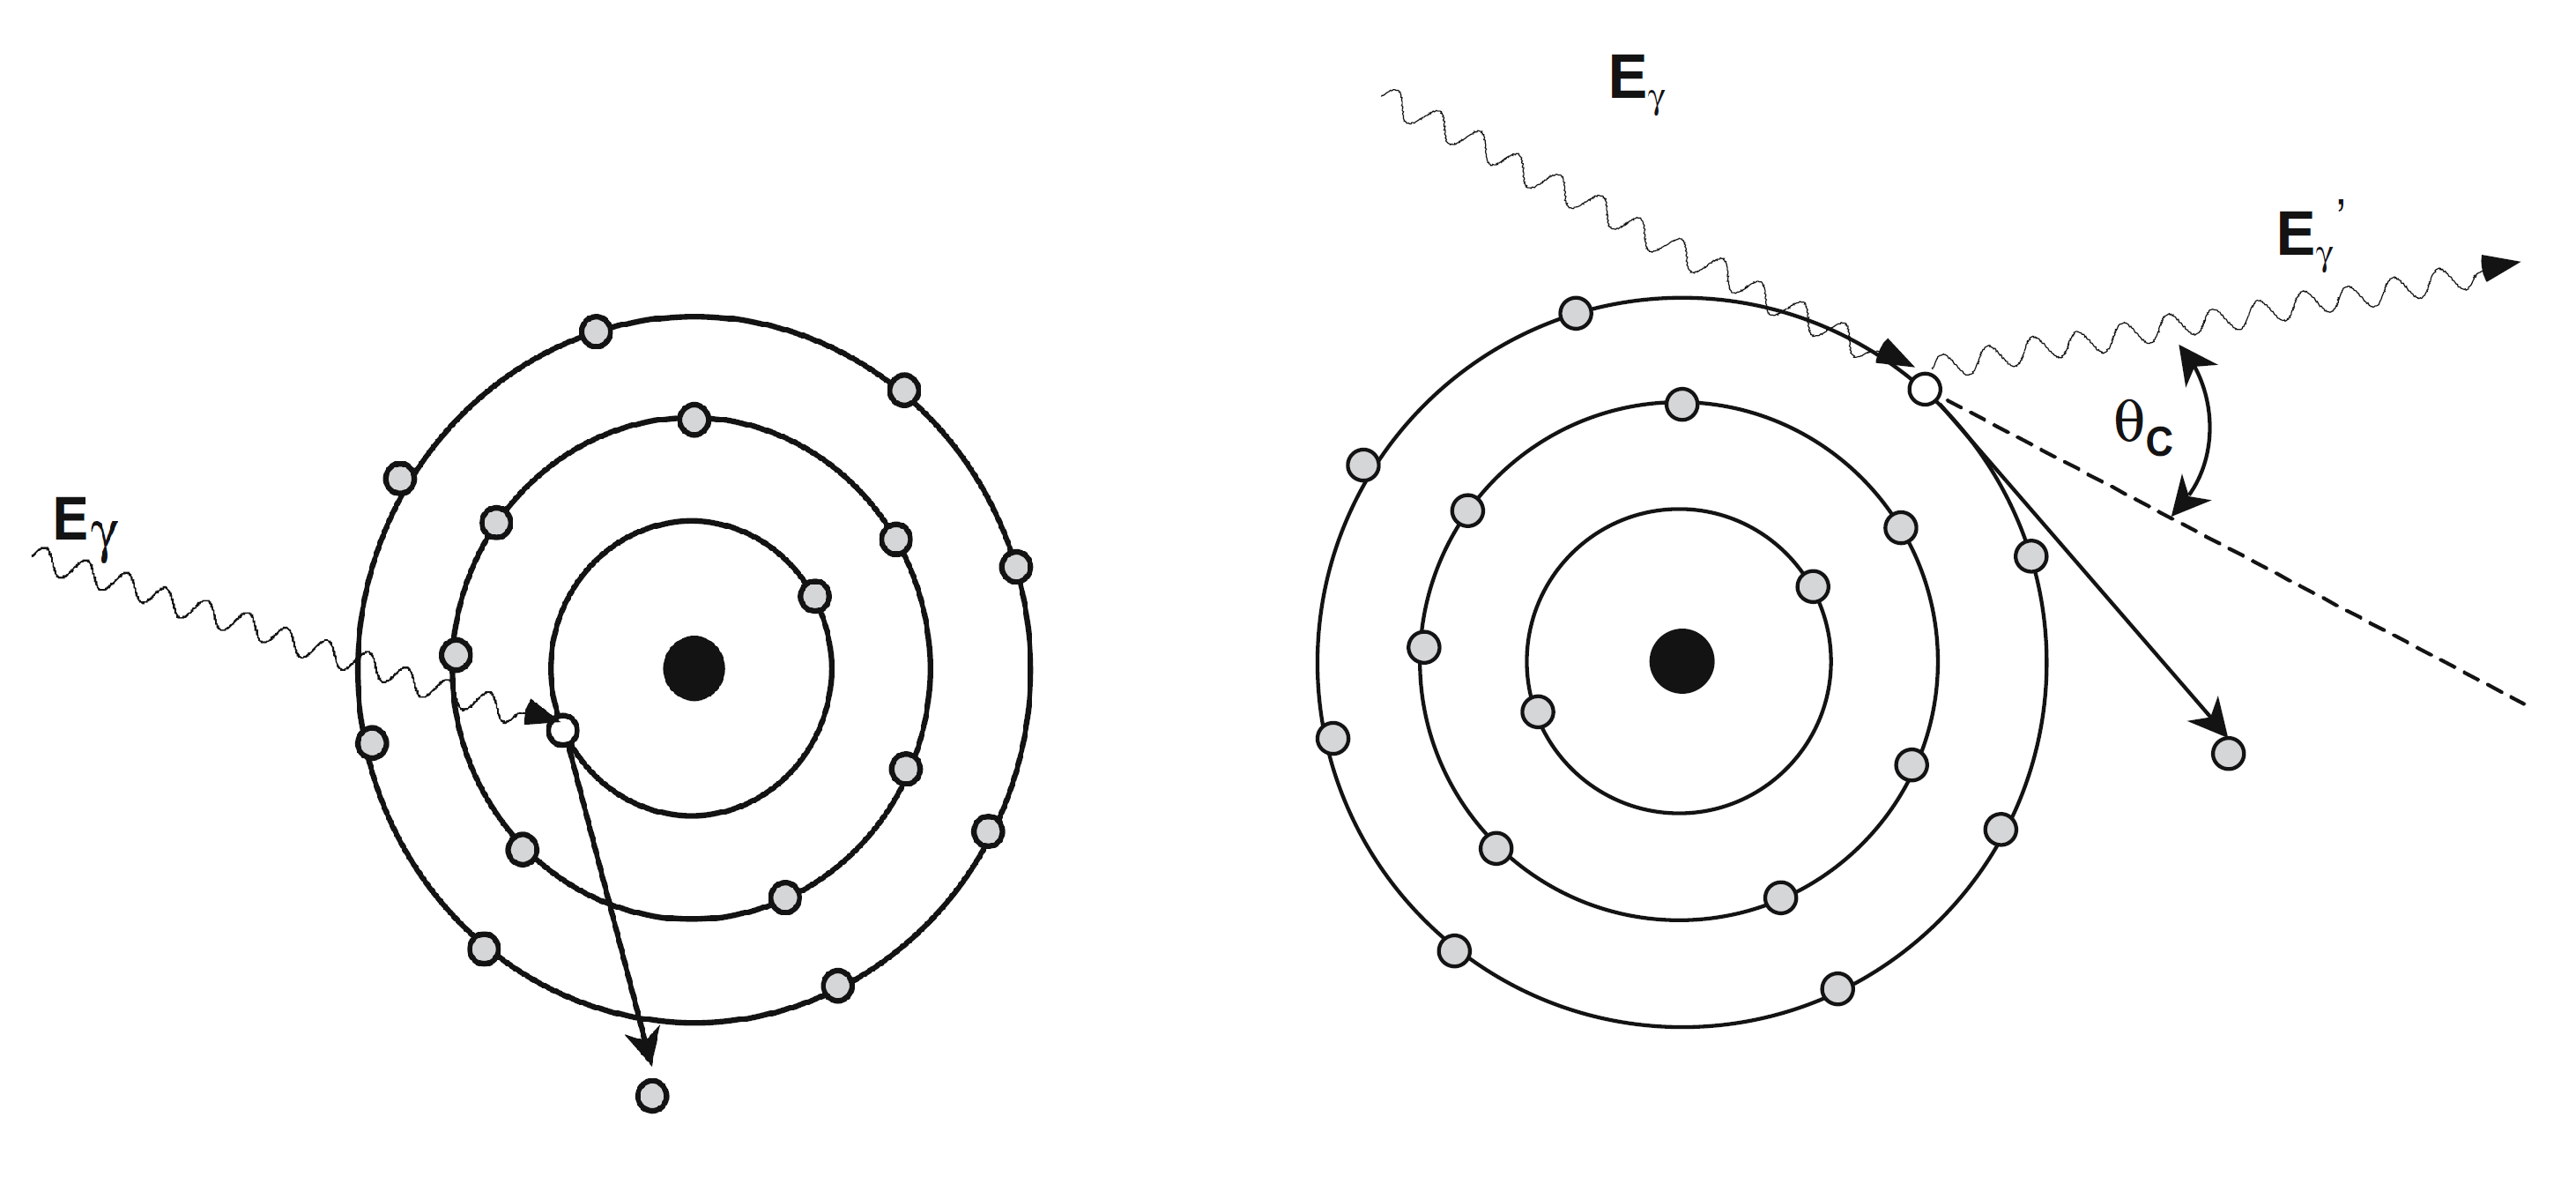
\includegraphics[scale=0.45,angle=0]{2_Theory_Methods/figures/Bailey_gamma_interactions.png}
\caption{The two main interactions of 511 \si{k\electronvolt} photons in matter, the photoelectric absorption (left) and Compton scattering effect (right)~\cite{Bailey2005}.} 
\label{fig_2:511_interactions}
\end{figure} 
%
\subsection{Attenuation}
Knowledge of the probabilities for interaction of the 511 \si{k\electronvolt} photons in a material can be used to calculate a precise attenuation factor that can be applied at the macroscopic level. Given a well collimated photon beam of intensity $I_0$, the intensity $I_x$ at depth $x$ within the material (along the direction of the beam) will be reduced due to interactions with the material acording to
\begin{equation} \label{Attenuation}
I_x = I_0 e^{-\mu x} \ ,
\end{equation}
where $\mu$ is the linear attenuation coefficient ( in $cm^{-1}$). This factor accounts for all possible interactions, whether absorption or scattering, and its value depends on the material properties and the energy of the photons.
%
Specifically for \gls{pet} where we are interested in the detection of both anihilation photons, the attenuation in the direction of the photon pair can be summed up, resulting in a factor that is independent of the depth of the annihilation and is only depended of the attenuation coefficient of the tissues or materials crossed by the line connecting the two photon detections and the total length of the line within the body, as shown in figure~\ref{fig_2:511_attenuation}~\cite{Phelps1975}. 

\begin{figure} [h!]
\centering
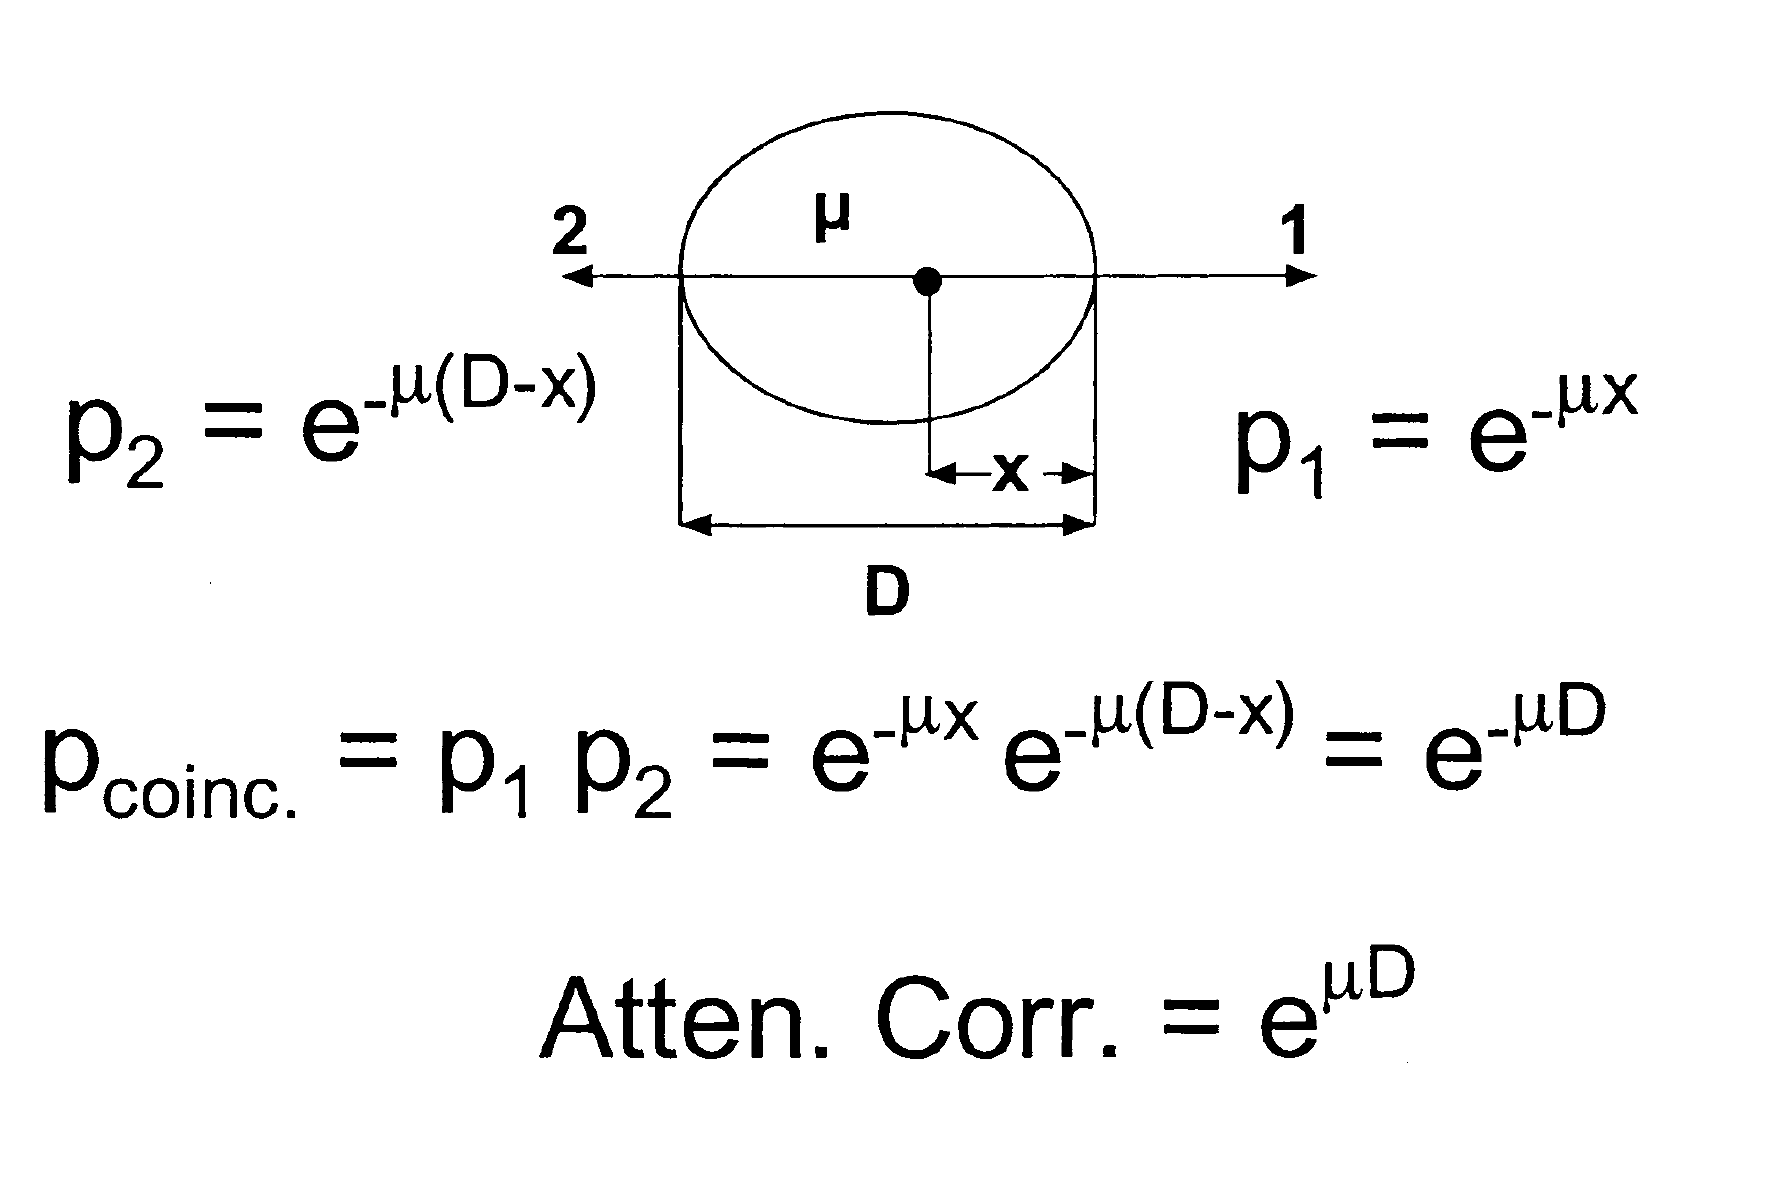
\includegraphics[scale=0.45,angle=0]{2_Theory_Methods/figures/Phelps_LOR_attenuation_correction.png}
\caption{Attenuation of LORs TODO:  to include in text ! } 
\label{fig_2:511_attenuation}
\end{figure} 

\section{PET Systems}

\subsection{PET Detectors}
The goal of a PET imaging system is to stop and detect the annihilation photon pairs and record information that can be used to estimate the annihilation event's position.
The basic component for the detection of annihilation gammas is the scintillation crystal. These are inorganic crystals that emit light (lower energy photons) upon interaction with the gammas. The amount of produced light is proportional to the energy deposited by the gamma interactions and can be used to deduce energy information of the interaction. Photosensitive detectors are coupled with the crystals to capture the produced light and output an electronic signal that can be digitally registered. Traditionally \glspl{pmt} are used in most PET systems, while some more recent systems make use of \glspl{sipm}. Depending on their mode of operation \glspl{sipm} can allow for better efficiency and response speed and can be used in conditions where \glspl{pmt} could not, such as within the MR field of PET-MR hybrid systems.
%
\footnotetext{https://www.radiologycafe.com/radiology-trainees/frcr-physics-notes/pet-imaging}
\begin{figure} [h!]
\centering
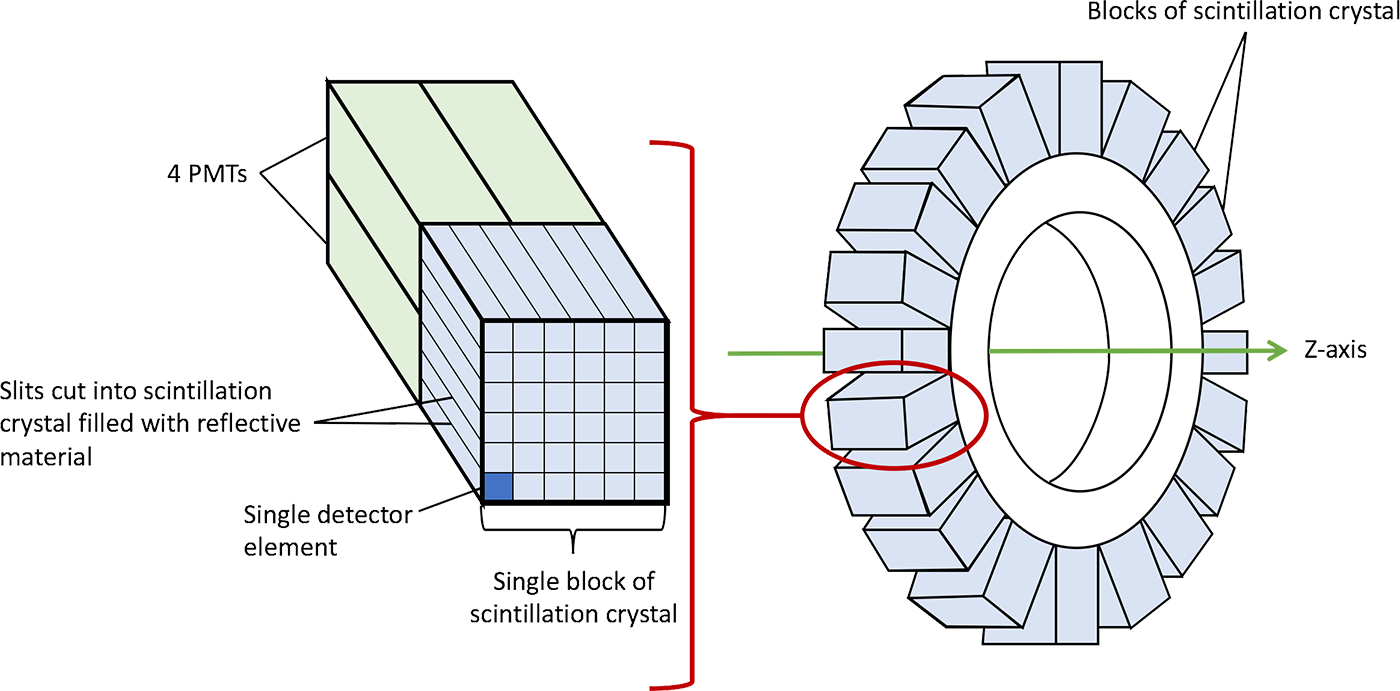
\includegraphics[scale=0.25,angle=0]{2_Theory_Methods/figures/block_detector.png}
\caption{Example PMT based block detector diagram and their placement within the PET ring (source: www.radiologycafe.com) } 
\label{fig_2:BlockDetectorAndRing}
\end{figure} 
\begin{figure} [h!]
\centering
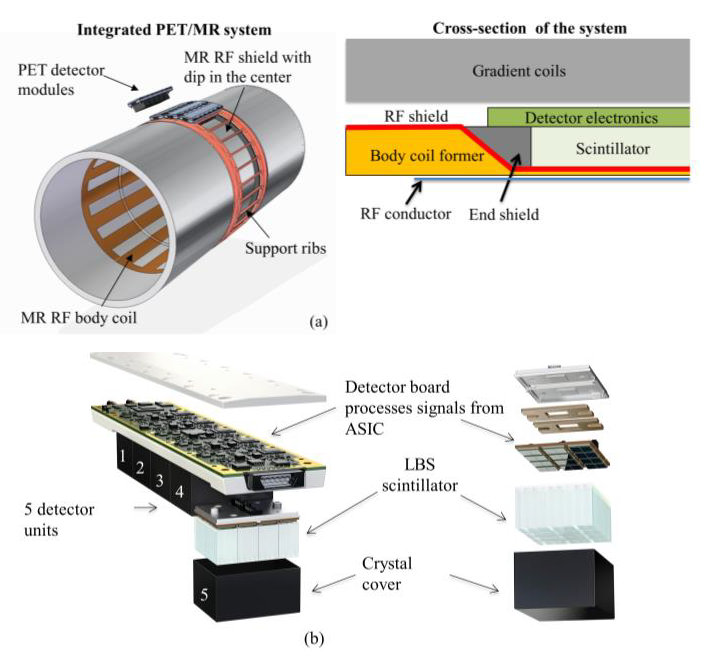
\includegraphics[scale=0.45,angle=0]{2_Theory_Methods/figures/SignaPETMR_Integrated_System.png}
\caption{Schematic of an hybrid PET-MR system with, comprising of detector module units (bottom) in a ring formation within the MR RF body coil (top)~\cite{Levin2016}.} 
\label{fig_2:SignaPETMR_Integrated_System}
\end{figure} 
%
%
%
The most common configuration of the PET detectors is within a block or module configuration, where a smaller number of photosensitive detectors to number of crystals is used. Examples are shown in figure~\ref{fig_2:BlockDetectorAndRing} for PMT based scanners and figure~\ref{fig_2:SignaPETMR_Integrated_System} for SiPMs within a hybrid PET-MR system. 
The blocks or modules are placed in ring configurations that provide full 360degrees of coverage in the transaxial direction. Multiple rings are often placed adjacent to each together to increase axial coverage and solid angle coverage that effectively increases the detection sensitivity. 

\subsection{PET Data coincidence sorting}
Individual events recorded by the detectors are called "single" events. In \gls{pet} detection of annihilation events requires the detection of both annihilation generated photons. To identify these photons the detection system makes use of "coincidence detection", which sorts pairs of single events detected within a predefined timing window as photons originating from an annihilation, or else true coincidence events. 
Due to uncertainties in the photosensitive detectors which result in timing uncertainly, a timing resolution τ is defined for the system.The coincidence timing window is then set at 2τ to sort pairs of events as coincidences.
As detectors and systems improve on timing resolution it now also possible to record the difference in arrival time between two coincidence photons, owing to the difference in distance travelled from annihilation to detection and the finite speed of light. That difference provides additional information for each detection, refereed to as \textit{time-of-flight} (TOF). This additional information can be used for better positional estimation of annihilation events across the \gls{lor}, as shown in figure~\ref{fig_2:TOF_bin}, resulting in improved reconstructed image quality and sensitivity.
%
%
\begin{figure} [h!]
\centering
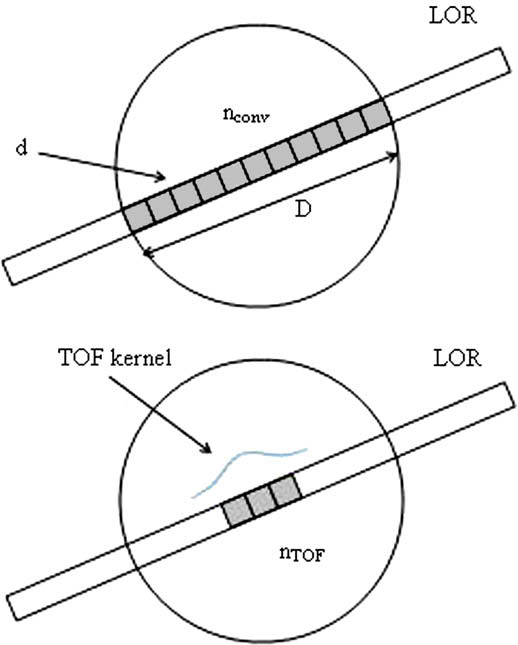
\includegraphics[scale=0.55,angle=0]{2_Theory_Methods/figures/TOF_bin.png}
\caption{Comparison of non-TOF (top) and TOF of annihilation event position across an LOR (bottom)~\cite{Conti2009}.} 
\label{fig_2:TOF_bin}
\end{figure} 
%
But not all events recorded within the coincidence window will always be originating from an annihilation event, they could also be one of the following. 
%
\begin{itemize}

\item\textbf{Random event}\\
As the rate of single events increases the chances of unrelated events being detected within the coincidence timing window are also increasing. In this case the system will record false coincidence events that are refereed as random events. 
The rate of random events is directly proportional to the size of the timing window and to the square of the activity in the scanner. These events are uncorrelated to the imaged object and hence degrade the acquired data and subsequently image quality and quantification.  
Randoms estimations can be made using the rates of single events or using delayed coincidence windows, which can then be applied as corrections during the image reconstruction process. 

\item\textbf{Scatter events}\\
As described scattering of the annihilation gammas results in a change of energy and direction. Subsequent detection of scattered gammas results in mis-positioned \glspl{lor} that also degrade the data, image quality and quantification. 
Because scattered gammas have lower energy than 511 \si{k\electronvolt}, they can be rejected by applying a lower energy threshold in the detectors. Due to energy resolution limitations this threshold is set to a low value that will result in some scatter events to be still recorded as coincidences. 
To correct for these events, special scatter simulation algorithms are employed to estimate the amount of scatter in the data and account for it during the image reconstruction process~\cite{Polycarpou2011}. 

\item\textbf{Multiple events}\\
Multiple events (more than two) can be are recorded within the coincidence timing window with no information on which of the events (if any) correspond to a true coincidence. As these cannot be used to resolve \glspl{lor}, they are commonly rejected completely or in some cases further processed to deduce which events are related to true coincidences using techniques that vary between scanner models and manufacturers. 
\end{itemize}
%
\begin{figure} [h!]
\centering
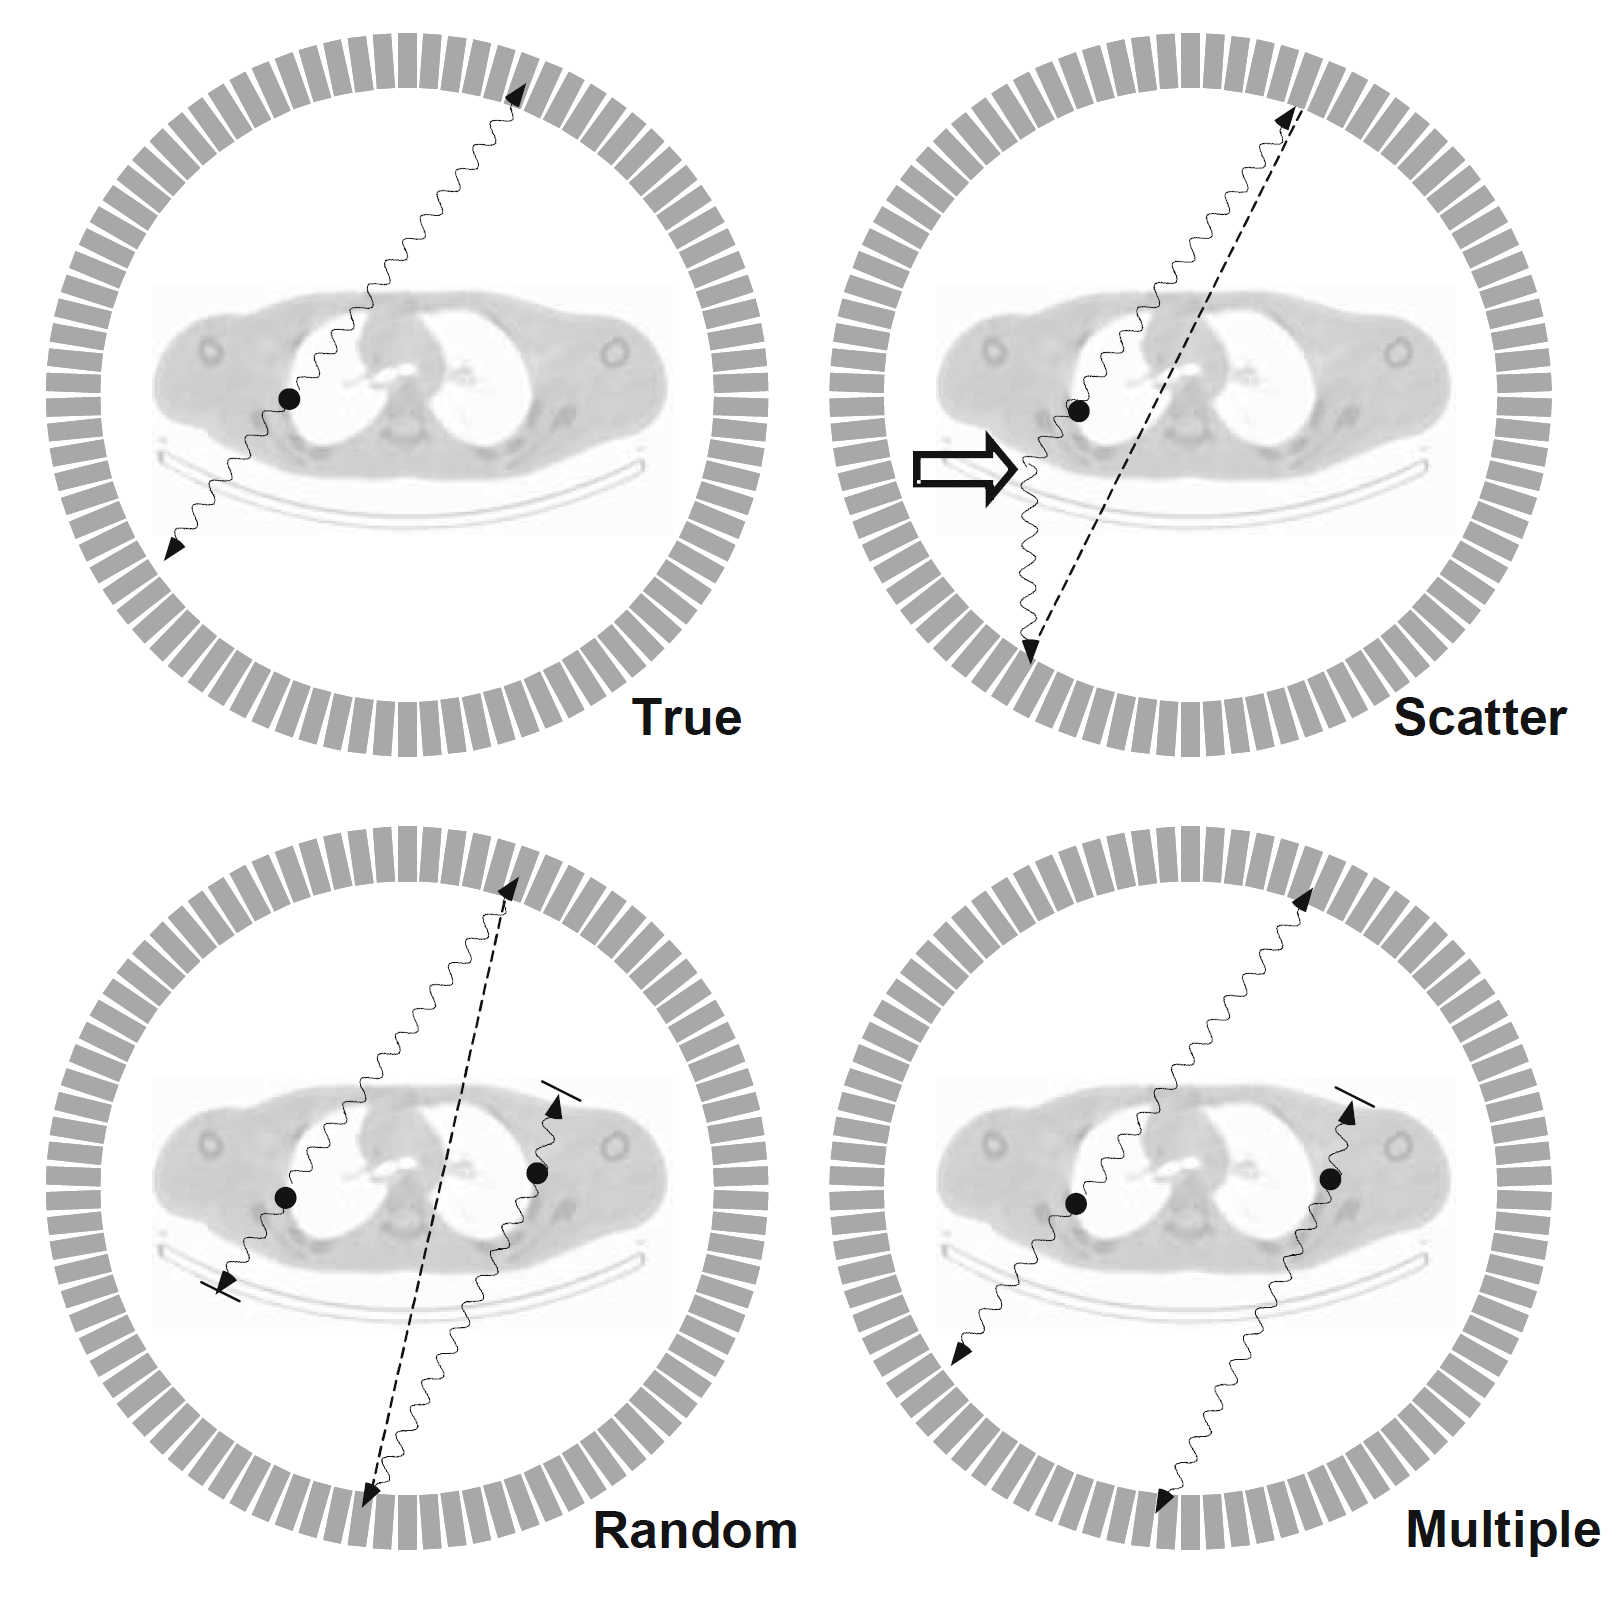
\includegraphics[scale=0.22,angle=0]{2_Theory_Methods/figures/Bailey_Scatter_Random_events.png}
\caption{Representation of different types of detected coincidence events~\cite{Bailey2005}. } 
\label{fig_2:BlockDetectorAndRing}
\end{figure} 
%
%
\subsection{PET acquisition}
As described the ring formation of PET detectors is the dominant geometry used in PET systems. Using multiple rings resuts in increase of axial \gls{fov}, solid angle coverage and possible combinations of detectors meaning higher number of ~\glspl{lor}. But early multi ring systems were making use of 2D acquisition, where only direct and cross-plane ring coincidences were allowed. 
This was enforced using tungsten septa between rings, as seen in figure~\ref{fig_2:2D3D}.The use of cross-planes allowed for the increase in axial resolution and the septa result in an uniform axial sensitivity profile as seen in figure~\ref{}. 

With evolving detector and electronics technology, 3D acquisition became possible and is now the standard acquisition mode. 3D acquisition offers the same data as 2D acquisition but also includes all the oblique \glspl{lor} data resulting in an increase of sensitivity (4 to 6 times)~\cite{Fahey2002}. The use of oblique views leads to non-uniform sensitivity profiles in the axial direction due to the higher number of \glspl{lor} closer to the center of the A-FOV, with the maximum sensitivity at the centre and a minimum at the edges of the axial \gls{fov}. A comparison between the 2D and 3D sensitivity on the same 45 direct planes is shown as an example in figure~\ref{fig_2:2D3DSensitivityProfiles}.
In addition to more coincidence events, the higher sensitivity and acceptance of events results to an increase of randoms scatter events, which now as well may be originating from activity outside the A-FOV of the system. 
%
\begin{figure} [h!]
\centering
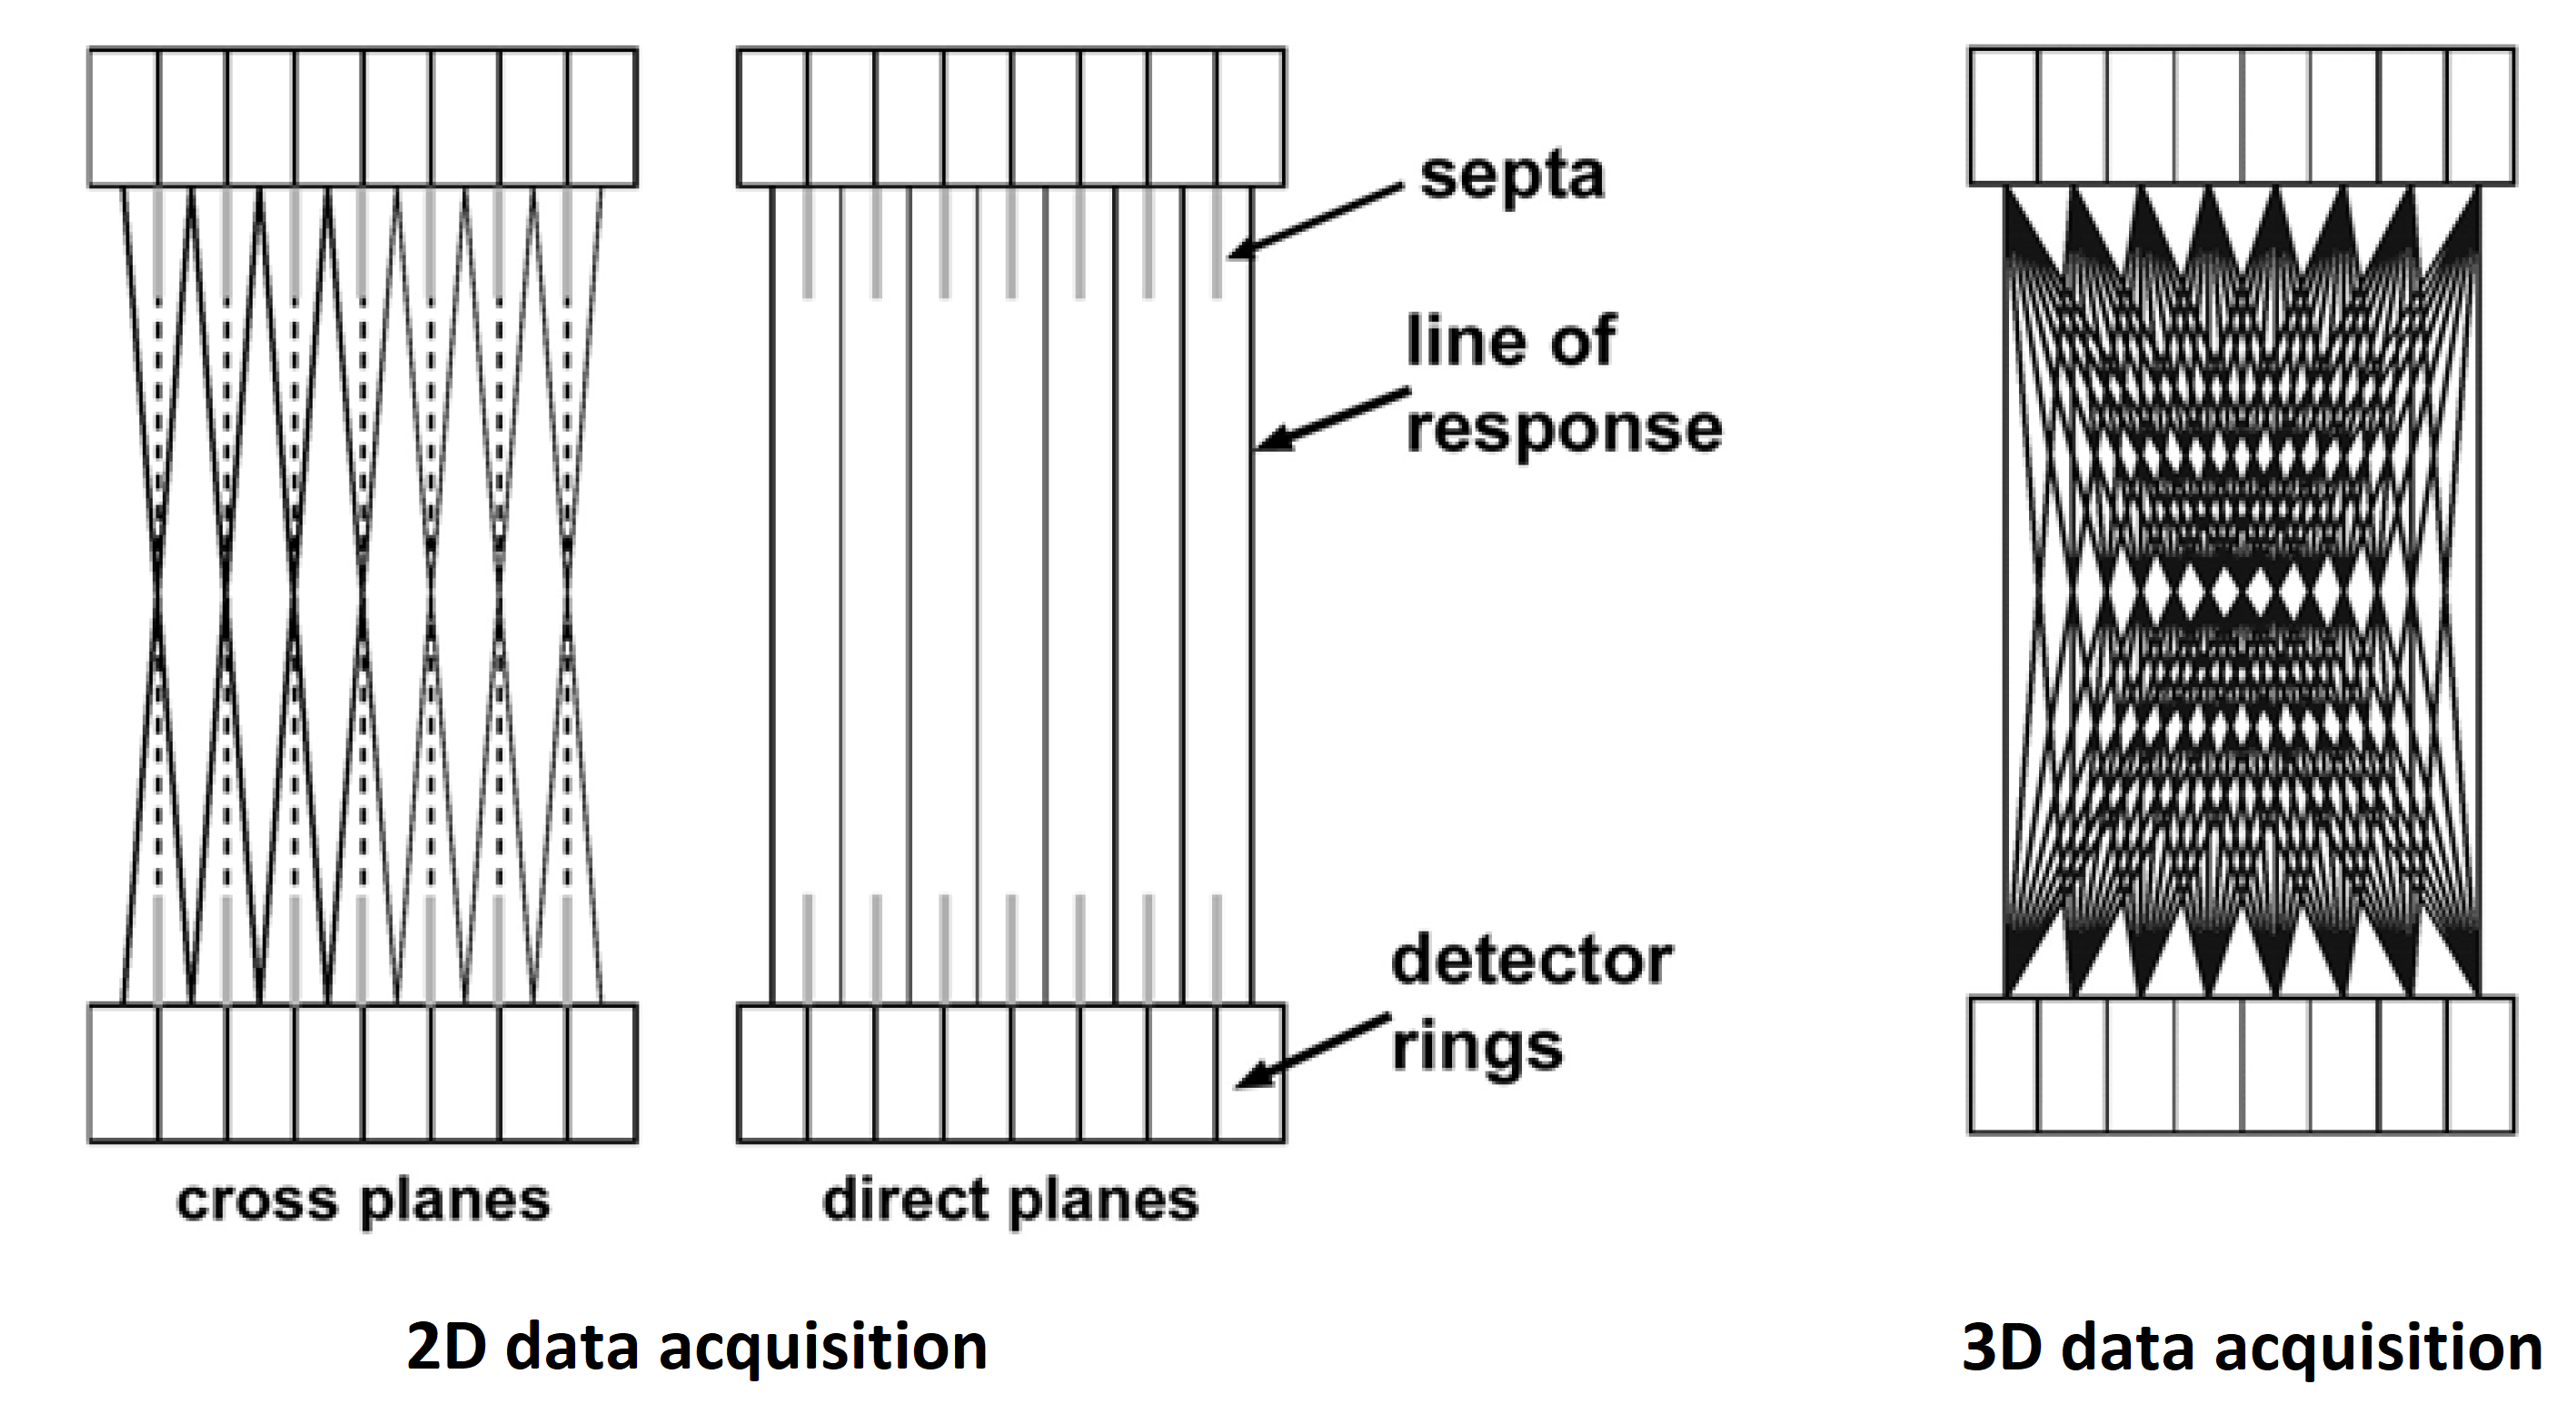
\includegraphics[scale=0.40,angle=0]{2_Theory_Methods/figures/Phelps_2D_3D_Acquisition.png}
\caption{Example of 2D (left) and 3D (right) acquisition mode LORs for an 8 ring scanner.} 
\label{fig_2:2D3D}
\end{figure} 
\begin{figure} [h!]
\centering
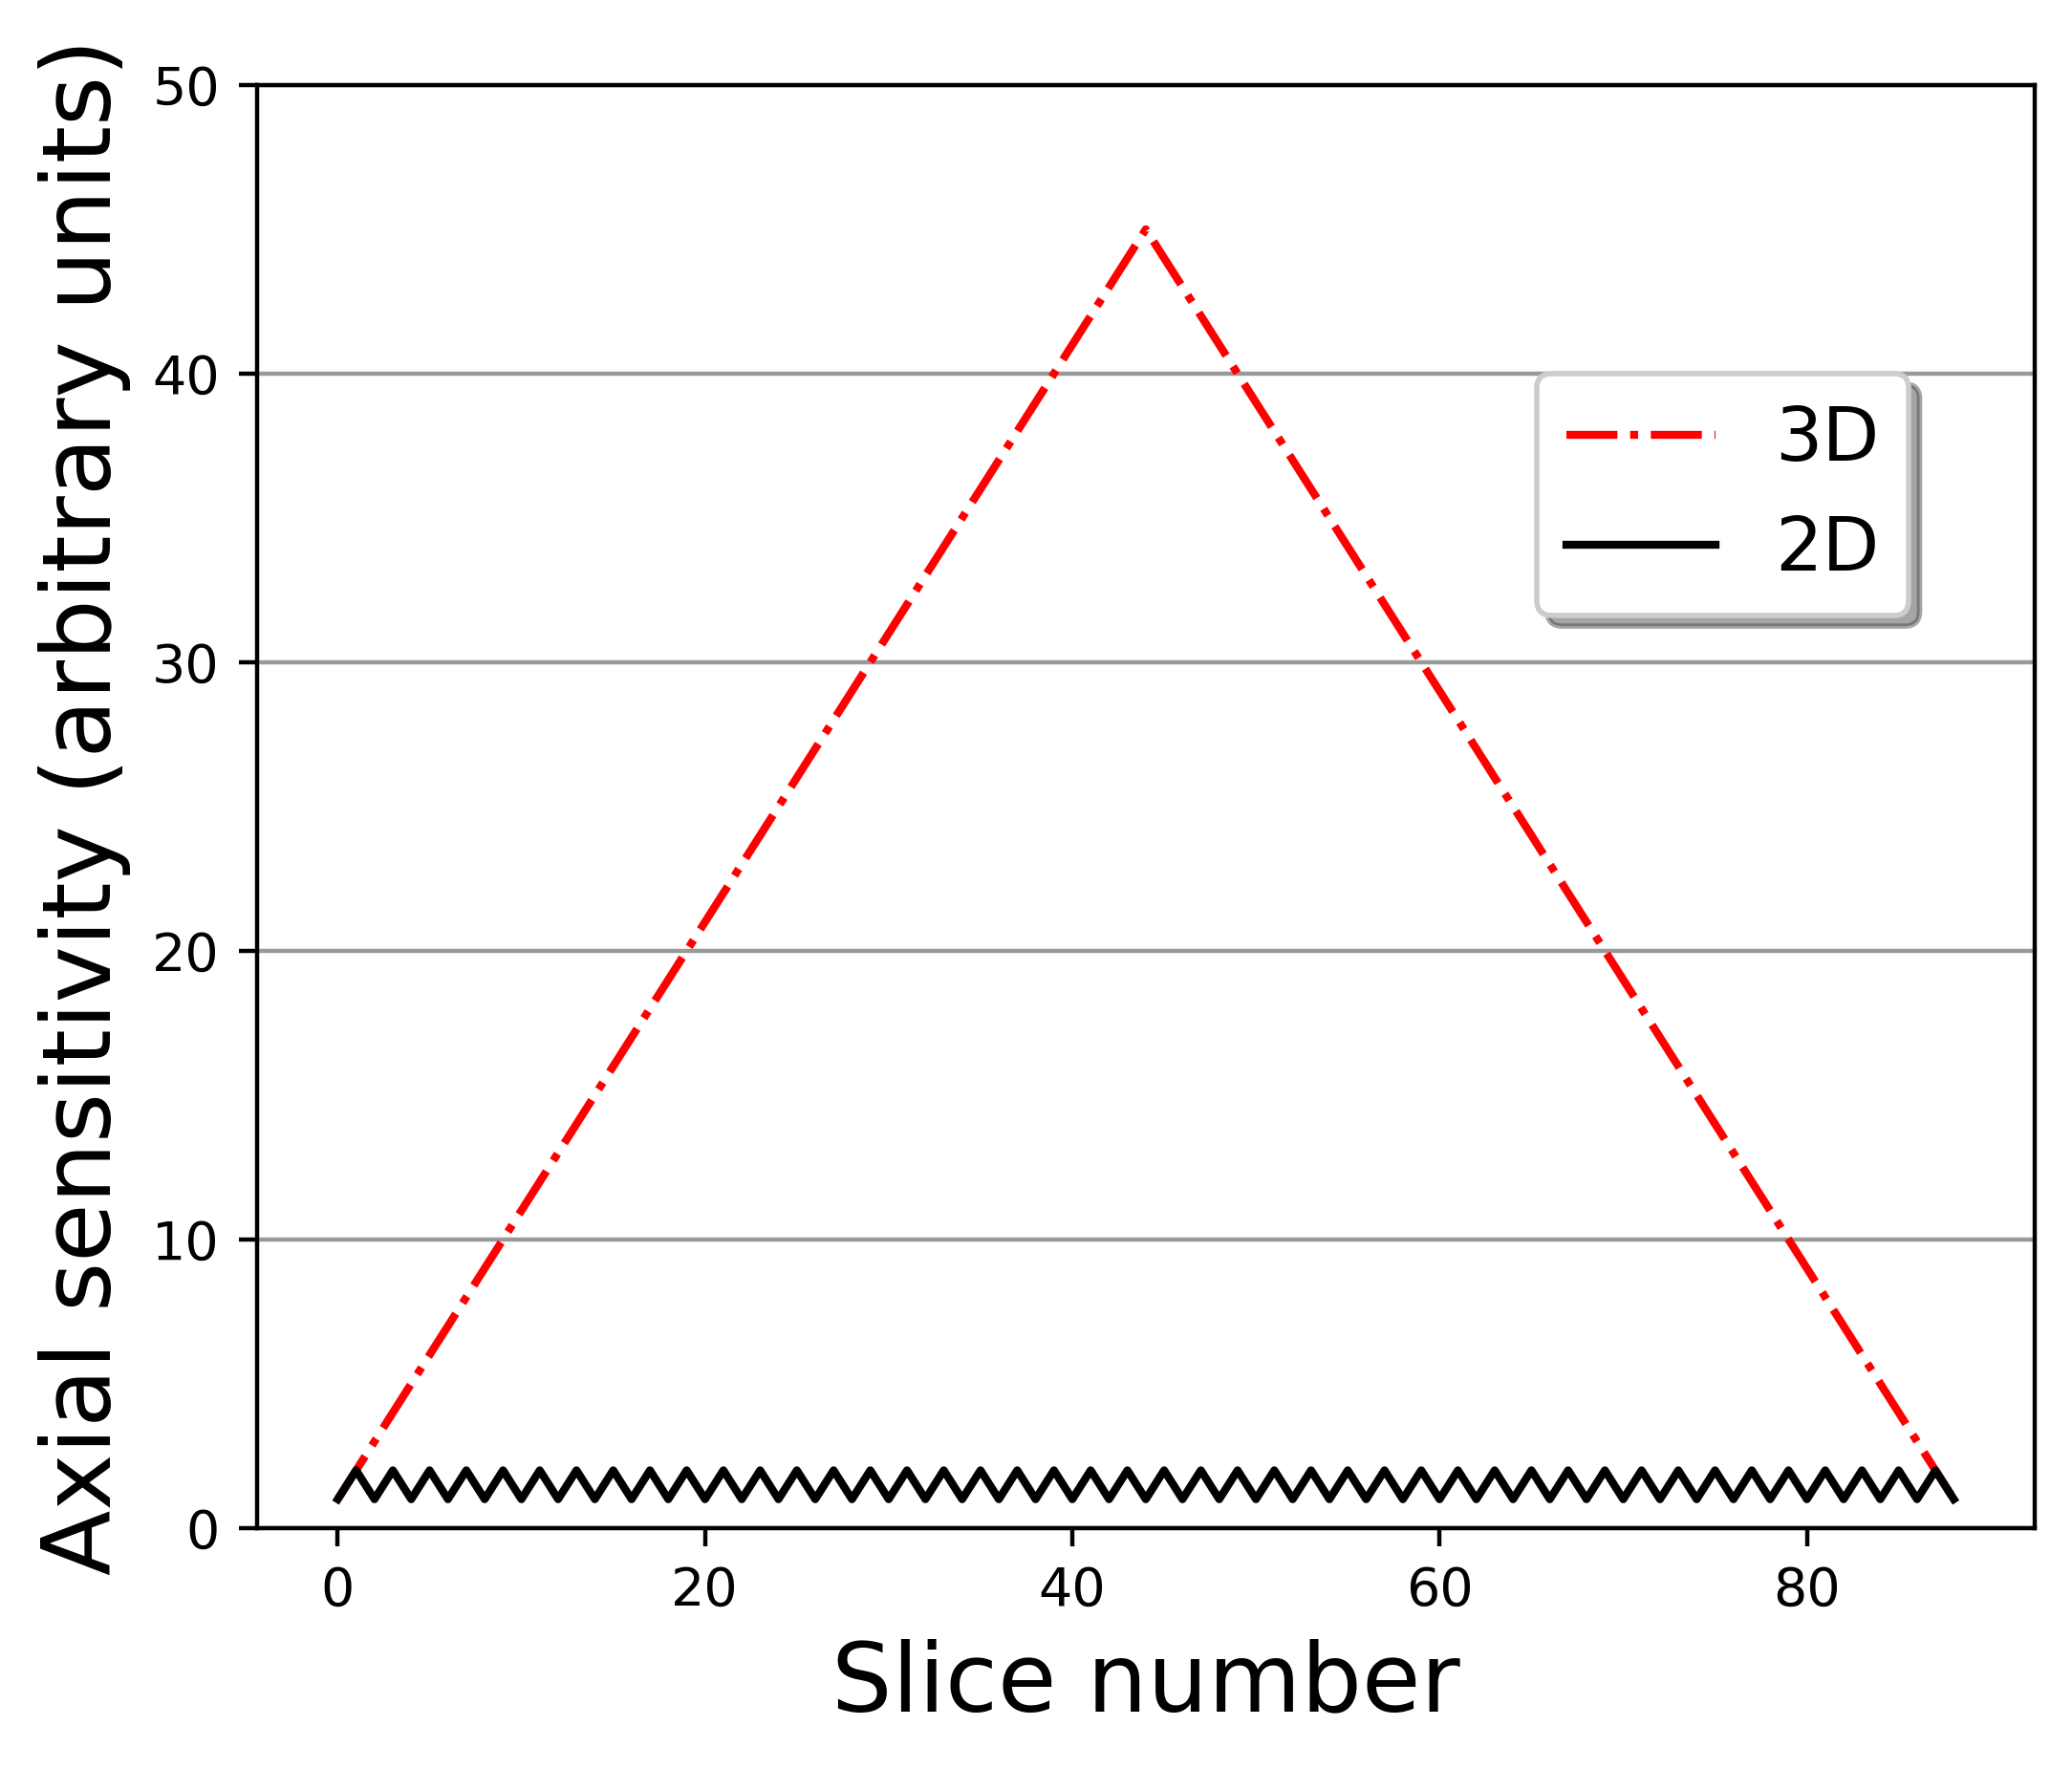
\includegraphics[scale=0.50,angle=0]{2_Theory_Methods/figures/2_2_2D3DSensitivityProfiles.png}
\caption{Example of 2D and 3D axial sensitivity profiles for a scanner with 45 direct planes.} 
\label{fig_2:2D3DSensitivityProfiles}
\end{figure} 
%
%
In 3D mode the maximum angle of events accepted in the axial direction can be sometimes limited by enforcing a maximum ring difference permitted \glspl{lor}. This results in a uniform axial sensitivity profile at a central region of the axial \gls{fov}.
%
In multiple beds acquisition, used to image objects with a length larger than the scanner A-\gls{fov}, in order to maintain an uniform axial sensitivity a degree of overlapping is used. This allows for the regions at the edges of the bed positions to be sampled in two bed acquisitions and even out the sensitivity of the combined acquisition. The degree of overlapping can vary, depending on requirements of sensitivity uniforming and speed of acquisition.
%
\subsection{Storage of PET coincidence events}
The recorded coincidence data are stored digitally to allow post processing and reconstruction of image data.
The different methods for storing the data can result to different storage requirements, allow or not allow for specific event information to be stored and even necessitate different reconstruction techniques. 

\begin{itemize}

\item\textbf{List Mode}\\
In the simplest form coincidence events can be stored in a binary file as a stream of events by the order of their detection. This format follows naturally the detection process and allows for multiple detector information to be included in each event. A time tag is normally included in the data stream every millisecond. The minimum information recorded per event is the detector pair IDs. Any additional information such as time-of-flight, detection energy etc. can also be included with each event.
The use of list-mode files is practical for dynamic studies as they takes less storage space than the other alternative formats described bellow, and furthermore they allows for subsequent re-binning into any required temporal framing. Reconstruction algorithms can be derived to reconstruct data directly using the list-mode stream.

\item\textbf{Histogram}\\
Coincidence events per detector pair (\gls{lor}) can be summed together and stored into a single entry. The total number of entries will be equal to the total number of detector pairs. These entries make up a histogram, where effectively all the events have been histogrammed into the detector pairs. No timing information is preserved and hence multiple histograms are required if data are recorded dynamically, in a predefined temporal binning. 
This format can result in smaller files for static imaging compared to list-mode, but in the case of dynamic imaging it frequently results in much larger total size of files as multiple detector pair entries are empty (zero) for some time frames. Furthermore if time-of-flight information is also available, separate histograms need to be created for each time-of-flight bin (discretization of the TOF resolution), which further increases the zero entries and storage requirements. 

\item\textbf{Sinogram}\\
Sinograms are representations of the data in projections though the process of a Radon transform~\cite{radon1917}. Each pixel of the sinogram represents the integral of events over a specific line though the image space. The name "sinogram" comes from the fact that a point source (off-centred) is represented as a sine wave in the sinogram, as seen in figure~\ref{fig_2:Sinogram}.
%
\begin{figure} [h!]
\centering
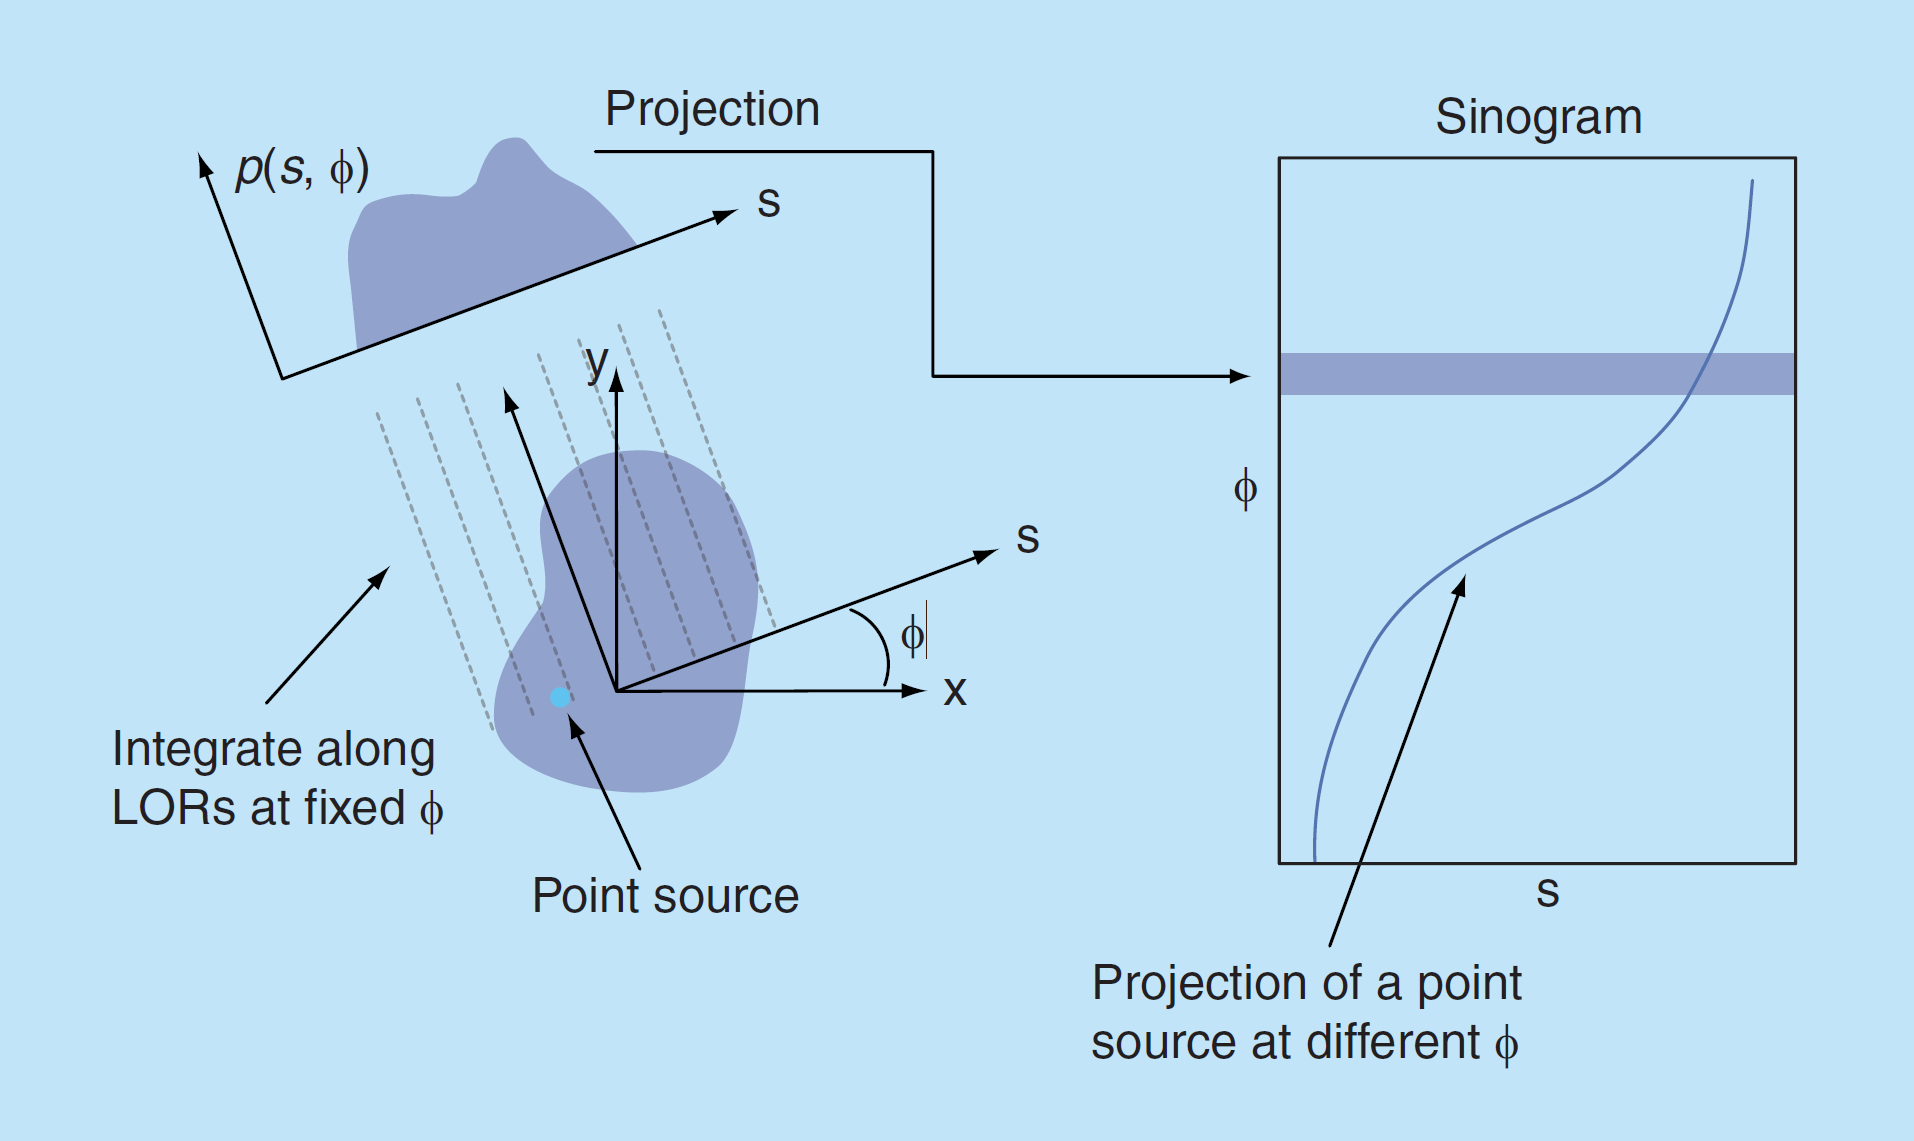
\includegraphics[scale=0.24,angle=0]{2_Theory_Methods/figures/Sinogram_Alessio.png}
\caption{Sinogram data representation though the process of integration across \glspl{lor} at an angle and example of point source representation~\cite{Tong2010}.} 
\label{fig_2:Sinogram}
\end{figure} 
%
Use of sinograms is inherited from other tomographic imaging methods where data are acquired as projections. In \gls{pet}, contrary to list-mode and histograms where the data are directly related to detector elements, conversion of data to sinograms requires certain processing steps. As seen in figure~\ref{fig_2:Sinogram_detector_to_Sino}, parallel \glspl{lor} at a specific direction are used to form the sinogram along a particular row. The sampling of the sinogram space will depend on the size of the sinograms required, and data conversions will be required  to match the required sinogram sampling \cite{Fahey2002}. 
%
\begin{figure} [h!]
\centering
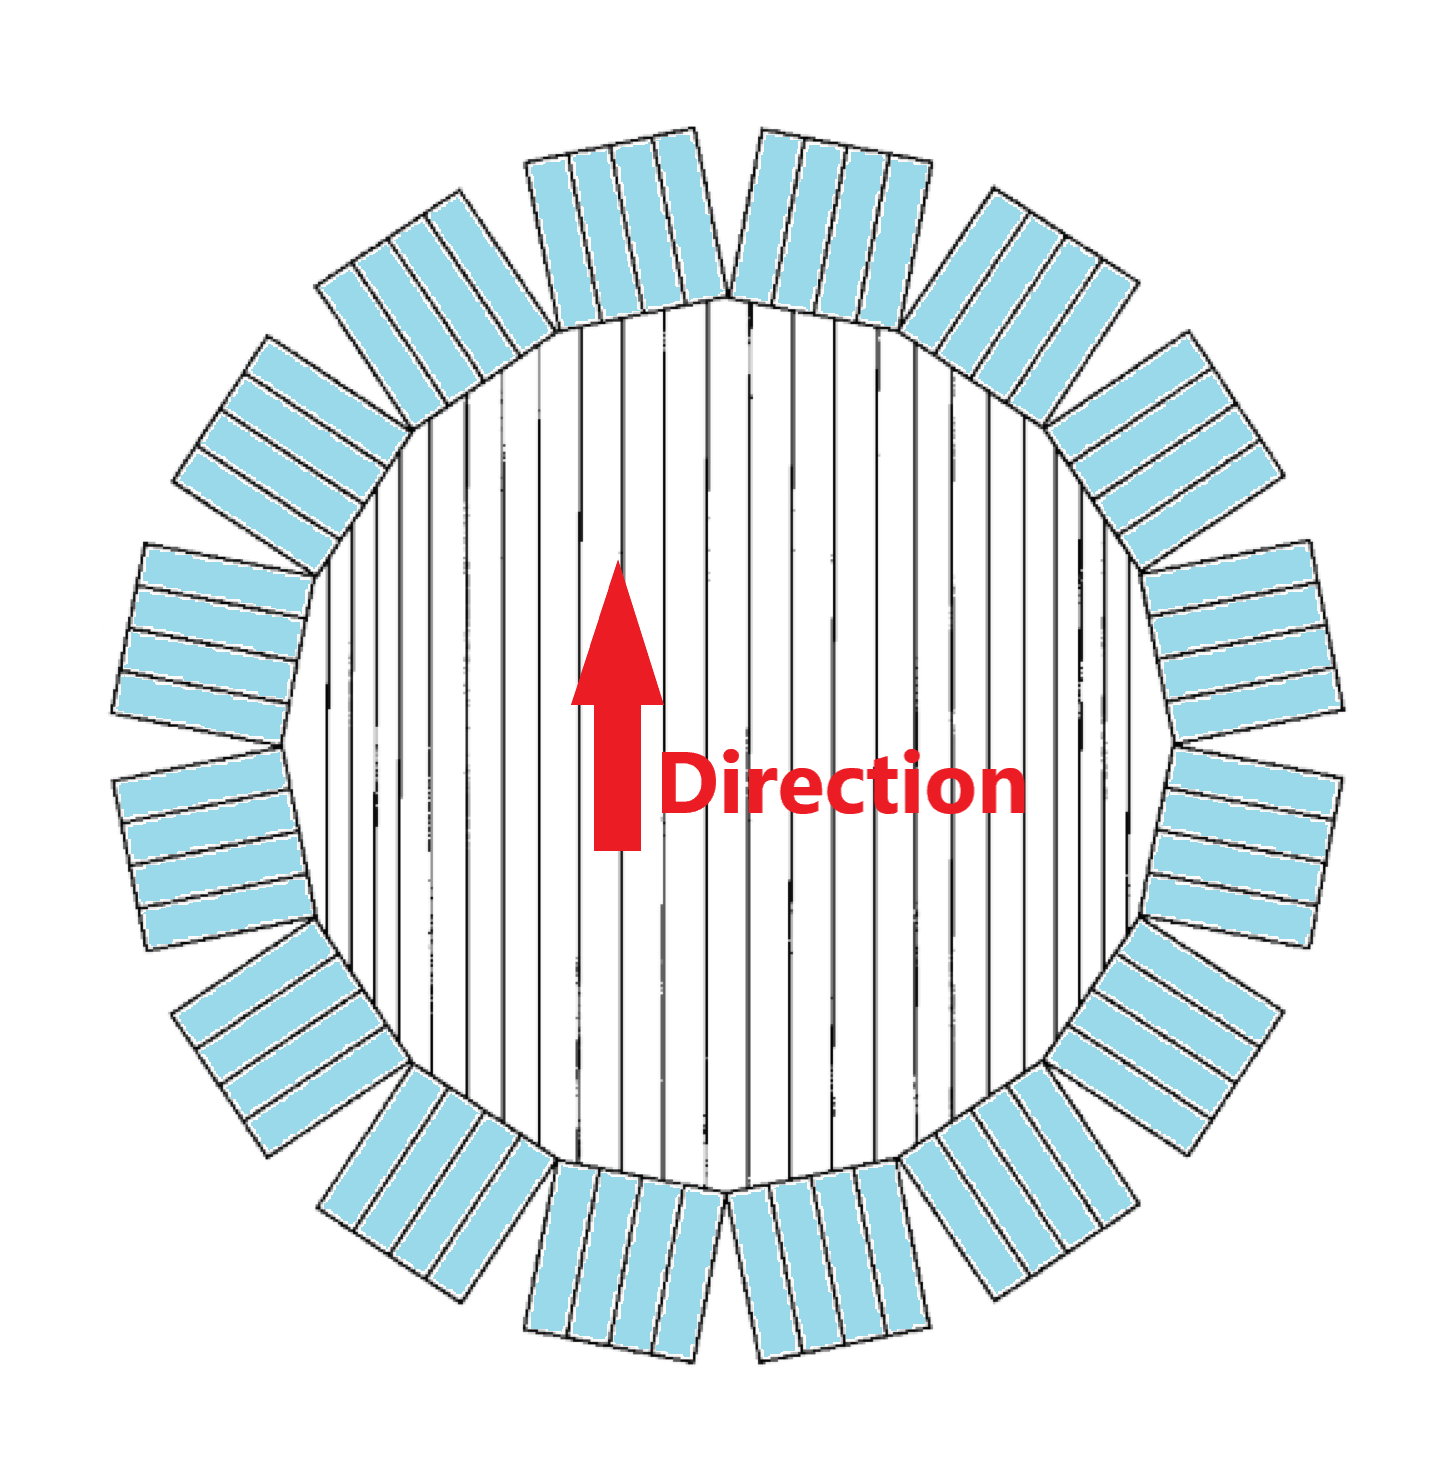
\includegraphics[scale=0.15,angle=0]{2_Theory_Methods/figures/Sinogram_detector_to_Sino.png}
\caption{Example projection though the PET field of view for a specific direction~\cite{Fahey2002}.} 
\label{fig_2:Sinogram_detector_to_Sino}
\end{figure} 
%
In practice events can be detected in any angle within the transaxial plane as well as the axial planes that are defined by the multiple detector rings that form the \gls{pet} system. In 3D acquisition, crystals from all rings (or under certain maximum ring difference limitations) are allowed to record coincidences. In this case the number of sinograms increases to allow all the possible co-planar angle combinations, and the radon transform is extended in 3D. With the introduction of time-of-flight information, a separate set of sinograms is required for each TOF bin and when dynamic data are captured a separate set per temporal bin. In practice different types of compression have been used to reduce the total size of sinogram raw data.

\end{itemize}

\subsection{PET Corrections and Quantification}

\begin{itemize}
\item\textbf{Randoms correction}\\
As discussed previously, an estimate of random events can be made using a sufficiently delayed coincidence window or by measurements of single event rates between all \glspl{lor}. The random rates are provided as a separate stream of events in list mode or in sinogram/histogram datasets and are used as additive corrections within statistical reconstruction methods. 
\item\textbf{Normalisation}\\ 
\Glspl{lor} will have slightly different sensitivity from others, due to detector and geometric efficiencies effects. Normalisation coefficients for each \gls{lor} are estimated using measurements and modelling of the normalisation components that form the normalisation coefficient, and are subsequently used in reconstruction to correct for these efficiencies.
\item\textbf{Dead-time correction}\\
After every detection event a certain amount of time is required for sub-systems involved in the detection to become ready for detection again and so interaction events occurring during that recovery time will not be registered. As the number of interactions increases at higher imaged activities, the proportion of events not registered is also increasing. This results is a non-linear system response for different levels of imaged activities. Dead-time correction is applied by the use of lookup tables and live dead-time monitoring measurements during acquisition.
\item\textbf{Scatter correction}\\
As described previously, a certain amount of the annihilation gammas will scatter with the atoms of the travelling medium via Compton scattering, which results in changes of energy and direction of the gamma. Even after energy filtering, an amount of those scattered gammas will be detected and recorded as coincidence events and degrade the PET data and affect image quality and quantification. The most commonly used approach to account for scatter in clinical scanners is the use of analytical simulation based scatter estimates. These simulations are based on an initial activity distribution estimate from the uncorrected PET data and knowledge of the probability of scattering. Scatter estimates, similar to random estimates, are used as additive corrections within statistical reconstruction methods.
\item\textbf{Attenuation correction}\\
Absorption or scatter interactions within the body result in loss of gammas detection. Even if one of the two annihilation gammas is lost the result is a non registered event and so the probability of attenuation depends on the total probability of interaction within a \gls{lor} and is independent of the annihilation position within that line. The attenuation factors within the body can be estimated using transmission measurements, either with radioactive sources or X-rays. For these measurements earlier scanners made use of positron or single gamma sources to estimate attenuation while most modern clinical systems make use of \gls{ct} or \gls{mr} scans. 
\item\textbf{Calibration Factor}\\
Contrary to other nuclear medicine techniques, \gls{pet} is fully quantitative and can be used to deduce absolute activity measurements from the reconstructed image data. For those measurements to be accurate a calibration factor needs to be set by cross-calibration measurements against a reference instrument. For dynamic studies where blood sampling is involved, it is also important to calibrate the scanner against the well-counter used for blood sample counting. The result of these measurement is a global calibration factor that converts detected counts to activity concentration. 
\end{itemize}


\section{Hybrid PET Systems}
As described above attenuation correction is essential for quantitative \gls{pet} imaging. Early \gls{pet} systems made use of external sources to acquire a transmission scan. Those would be either positron sources or single photon sources. Some of the drawbacks of these methods were that transmission scans would contribute to an increase of image noise on PET images and that transmission scan acquisition was increasing the total duration of the examination. 
Apart from attenuation correction the transmission scan was also used to find anatomical landmarks for correlation with findings in the PET scans. In clinical practice image fusion is preferred when possible, to combine information from CT and MRI scans with PET when those are available. 
These needs led to the development of hybrid PET systems, with the first PET/CT system being introduced in late 1990s and the first simultaneous PET/MR system in 2010~\cite{Townsend2008}. [Find PET/MR Reference]

\subsection{PET-CT}
The birth of hybrid PET/CT was driven by the clinical need of anatomical information needed to improve the diagnostic examination provided by functional images that PET provides. The first PET/CT prototype was designed with this aim in order to provide clinical quality CT with clinical quality PET~\cite{Townsend2008}. The first PET/CT was able to acquire a whole body PET/CT scan within an hour with precisely co-registered CT and PET images that were acquire close in time~\cite{Beyer2000}. The CT scan was also used for PET attenuation correction via scaling of attenuation factors that were measured for the CT X-ray energy to \si{k\electronvolt} of annihilation photons~\cite{Kinahan1998}. PET/CT eliminated the requirement for an additional transmission scan and the problems with added noise associated with transmission images. 

\subsection{PET-MR}
MRI provides anatomical images with higher soft-tissue contrast from CT imaging. The option of different acquisitions sequences allow for different type of MR imaging to be performed, which also includes functional MR imaging applications such as perfusion, diffusion, and spectroscopy for metabolites imaging. 
The fusion of PET and MR was challenging due to interference between the two systems~\cite{Disselhorst2014}. The use of PMT based detectors was possible only with long optical fibbers that shifted the detection of events at a distance away from the centre of the magnetic field~\cite{Shao1997,Mackewn2010}, while advancements with SiPM based detectors allowed for development of PET inserts~\cite{Kolb2012} and development of fully integrated PET-MR systems that perform synchronous acquisitions~\cite{Delso2011,Grant2016,Levin2016}.

!For the Signa PET/MR a total of 89 2.78 slices are imaged per bed position, using the set of xxx crystals. !

\section{Whole Body \& Total Body PET}
For many clinical applications as for example in oncology, PET imaging over the whole body is essential for detection and characterisation of metastatic disease. Developments in PET detectors technology and reduction of production costs has resulted in increasing axial length of PET scanners, with current widespread use of models(in 2021) offering between 10 to 26 cm of axial coverage.
A typical whole body examination will actually cover about half of the body , from base of the skull to the knees, and can be accomplished with as little as 5 bed positions and within a total examination time of 30 minutes. Certain diseases in oncology require full whole body coverage, in which case more bed positions are added and additional time is taken. 
The desired whole body coverage is achieved with acquisition of multiple bed positions, shifted in the axial direction. With scanners operated in 3D acquisition mode and the resulting varying axial sensitivity profile, the bed positions have to be overlapped to result in an even sensitivity profile and similar image noise across axial slices in the reconstructed PET images. 

\section{Static WB PET}
The first suggestion and optimization work in extending the effective A-FOV of PET scans using multiple bed positions was by made by Dahlbom \textit{et al.}~\cite{Dahlbom1992}. This work was made on PET systems operated in 2D mode, where a bed displacement of approximately equal to the system A-FOV was used to increase the acquisition effective A-FOV. As systems became capable of acquiring in 3D mode, which offers increased sensitivity but results in axial varying sensitivity profiles, different strategies were needed for multi-bed acquisitions. The two methods suggested and developed are the \textit{Step and Shoot}(SS) and the \textit{Continuous Bed Motion}(CBM) acquisition methods. 

\subsection{Step and Shoot}
\label{WB_Static_SS}
The SS method makes use of multiple bed positions that are partially overlapped in the axial direction to increase the sensitivity of the acquisition at the edges of each bed's FOV, by combining data of adjacent beds over the overlapping region as shown in figure~\ref{fig3_1:fullOverlap}. One way of combining the multi-bed datasets is to reconstruct each bed individually, displace the reconstructed images according to their axial location and combine them using weighted averaging~\cite{Schubert1996}. This method has prevailed in clinical PET systems that use the SS acquisition method, as it does not require addition considerations in the reconstruction process of each bed and the combination of bed images can be performed post-reconstruction. Alternatively the axial displacement of each bed raw dataset can be performed during the projection and back-projection process in iterative reconstruction, which then directly results in the reconstruction of the whole-body image~\cite{Ross2004}. Use of the overlap data in iterative reconstruction can potentially result to improved noise characteristics at the overlapping regions, as the full sampled statistics over these regions are combined prior to each image update~\cite{Ross2004,Stute2014}. 
%
\begin{figure} [ht!]
\centering
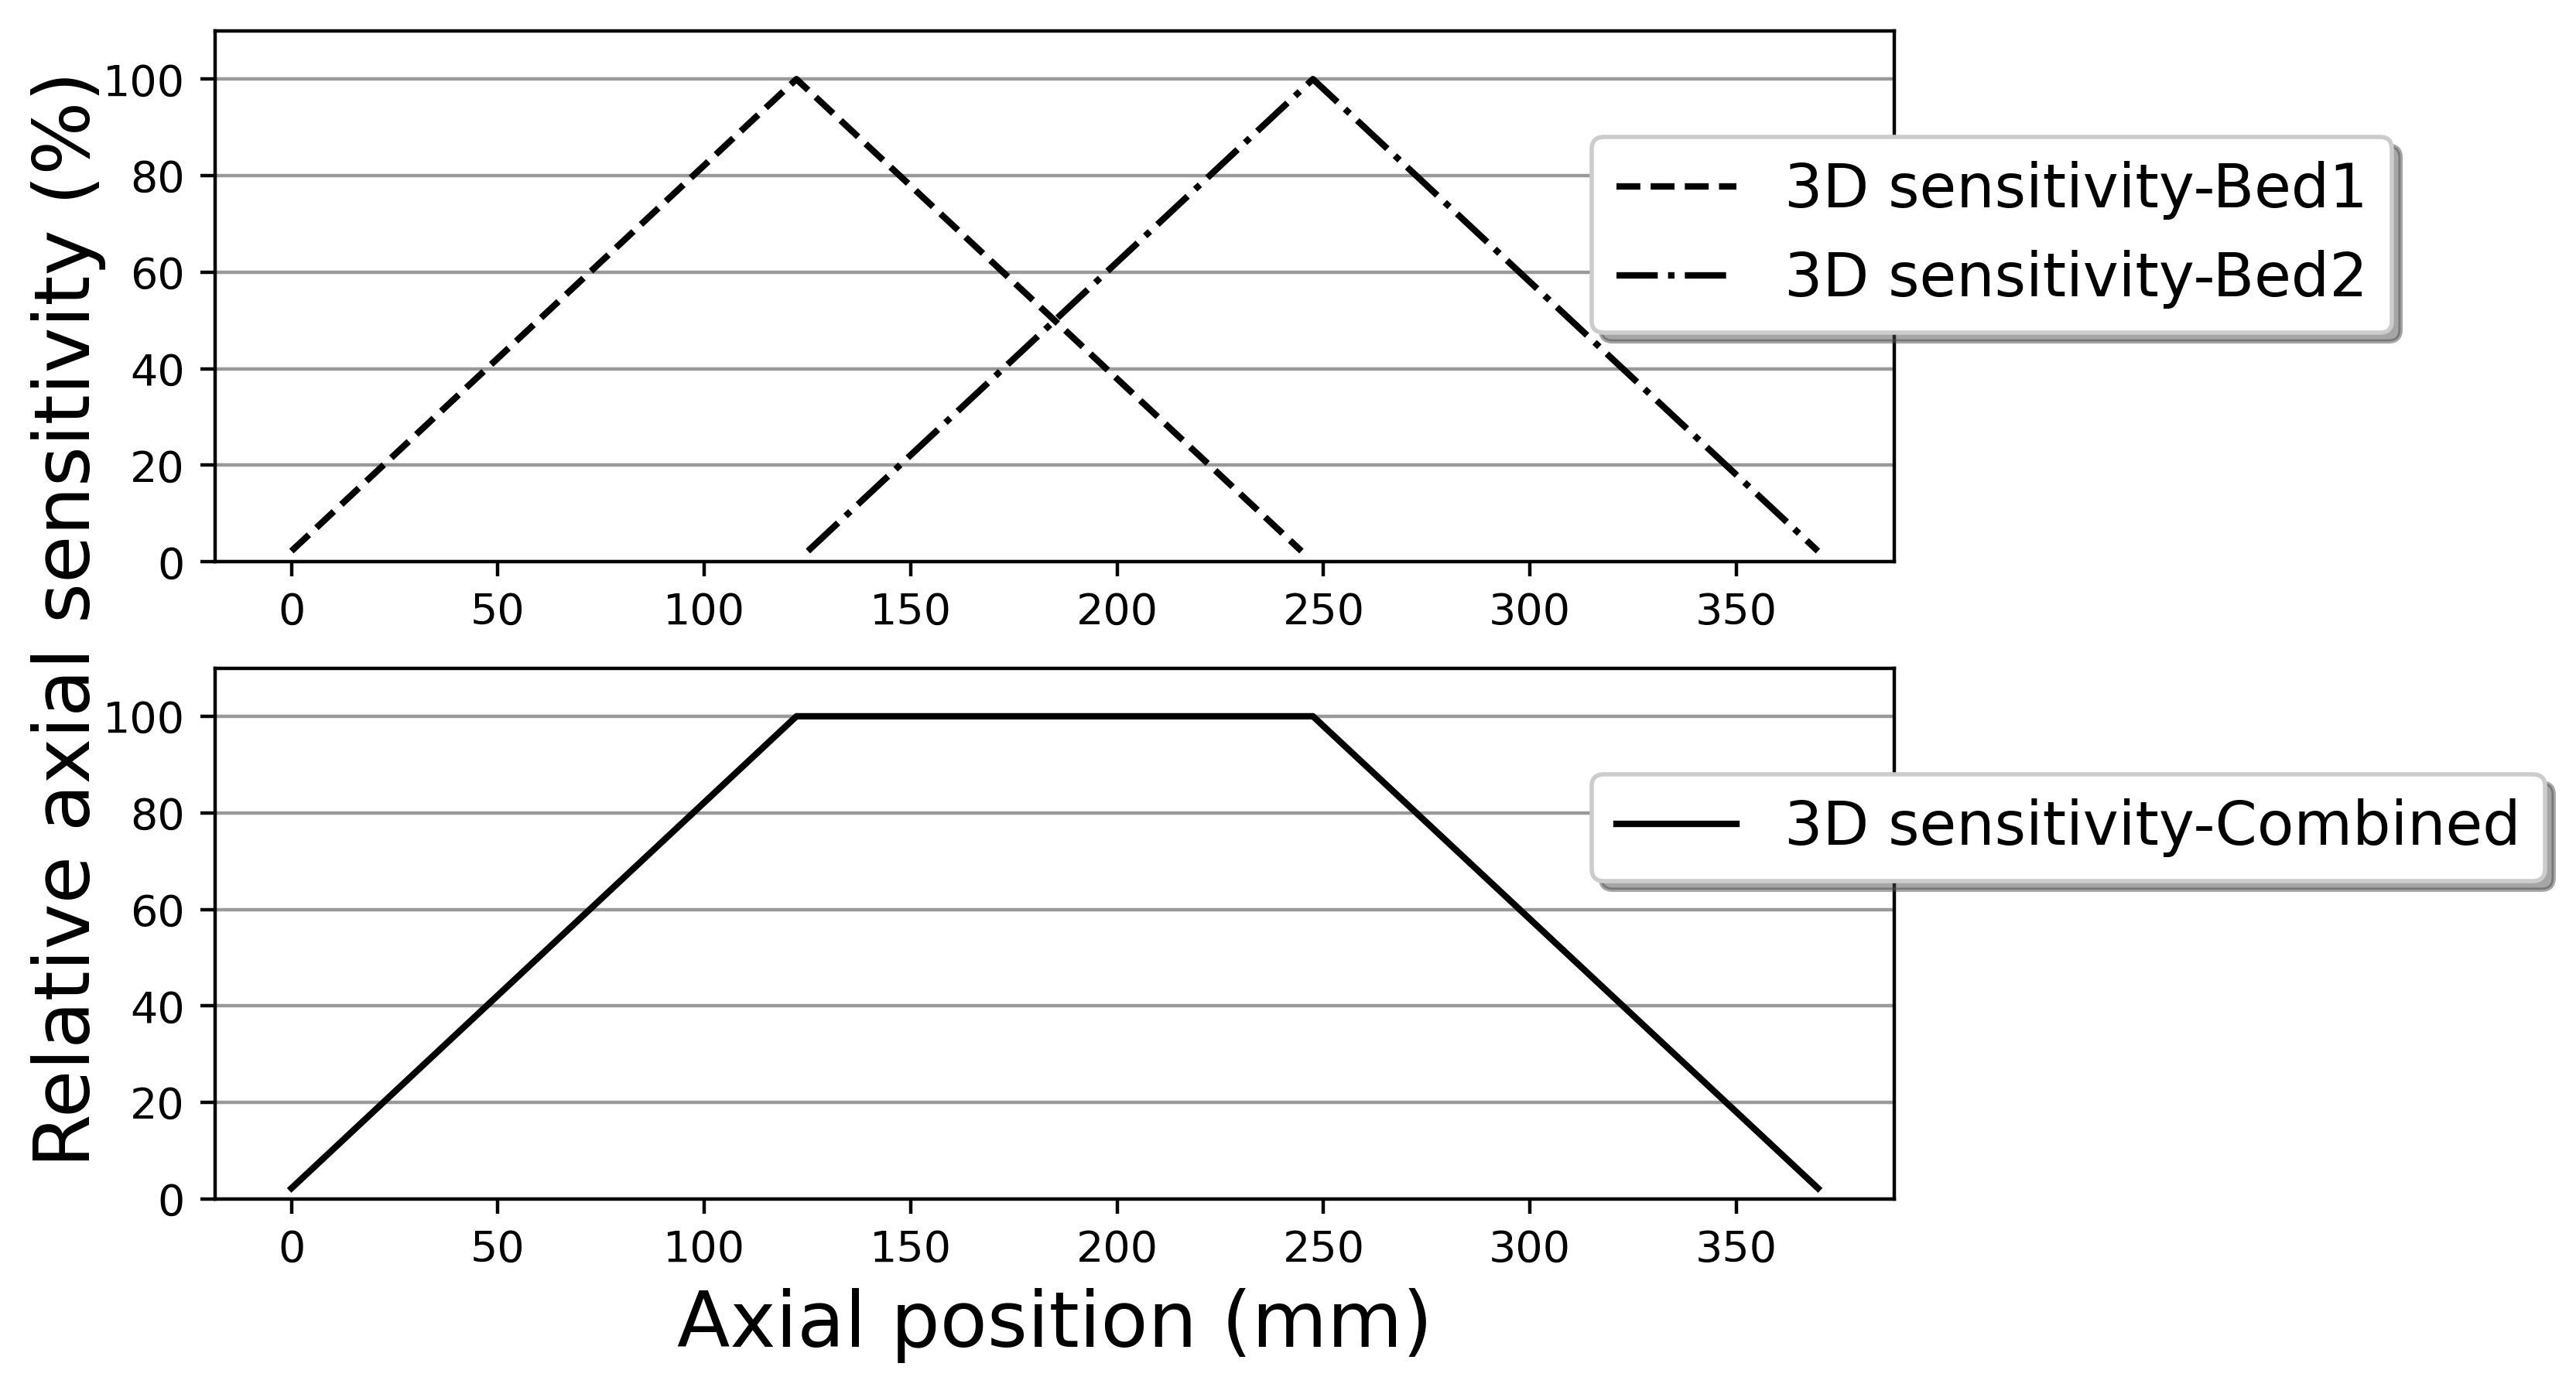
\includegraphics[scale=0.5,angle=0]{3_Results/3_1_DWB_Optimization/figures/SensitivityProfiles_fullOverlap.png}
\caption{Relative axial sensitivity of individual beds (top) and combined sensitivity profile (bottom) for approximately 50\% overlap.} 
%TODO: Add over-scan in the CBM D-WB protocols. 
\label{fig3_1:fullOverlap}
\end{figure}
%
The amount of overlap is a parameter to select according to the needs of the axial sensitivity profile.  The axial sensitivity profile for the Signa PET-MR system is shown in figure~\ref{fig3_1:fullOverlap}, where for a completely uniform axial sensitivity profile an overlap of 44 slices (\sim50\% of A-FOV) is required.
The amount of overlap used depends on the needs for uniformity in axial sensitivity and reconstructed image noise. This in term will also depend on the used reconstruction type and the activity distribution of the imaged subject~\cite{Schubert1996}. 
For standard clinical scanning at the Signa PET-MR an overlap of \sim27\% is used by default, to balance between sensitivity uniformity and examination time for standard WB examinations. The trade-off is made to accommodate longer effective A-FOV in the same acquisition time or to reduce acquisition time by use of less bed positions to image the same scan length. Examples of three overlapping options and the provided coverage are shown in figure~\ref{fig3_1:decreasingOverlap} and~\ref{fig3_1:BodyCoverage} figure respectively.
Many clinical WB protocols actually require imaging of approximately half the length of the body, from head to thighs, which can be accommodated with 5 or 6 bed positions. When full body coverage is required the number of beds is increased to 9 or 10. In DWB acquisitions where fast scanning is crucial the overlap can be decreased to maintain the same coverage with a lesser number of bed positions, as shown in option(C) of figure~\ref{fig3_1:BodyCoverage}. 
%
\begin{figure} [ht!]
\centering
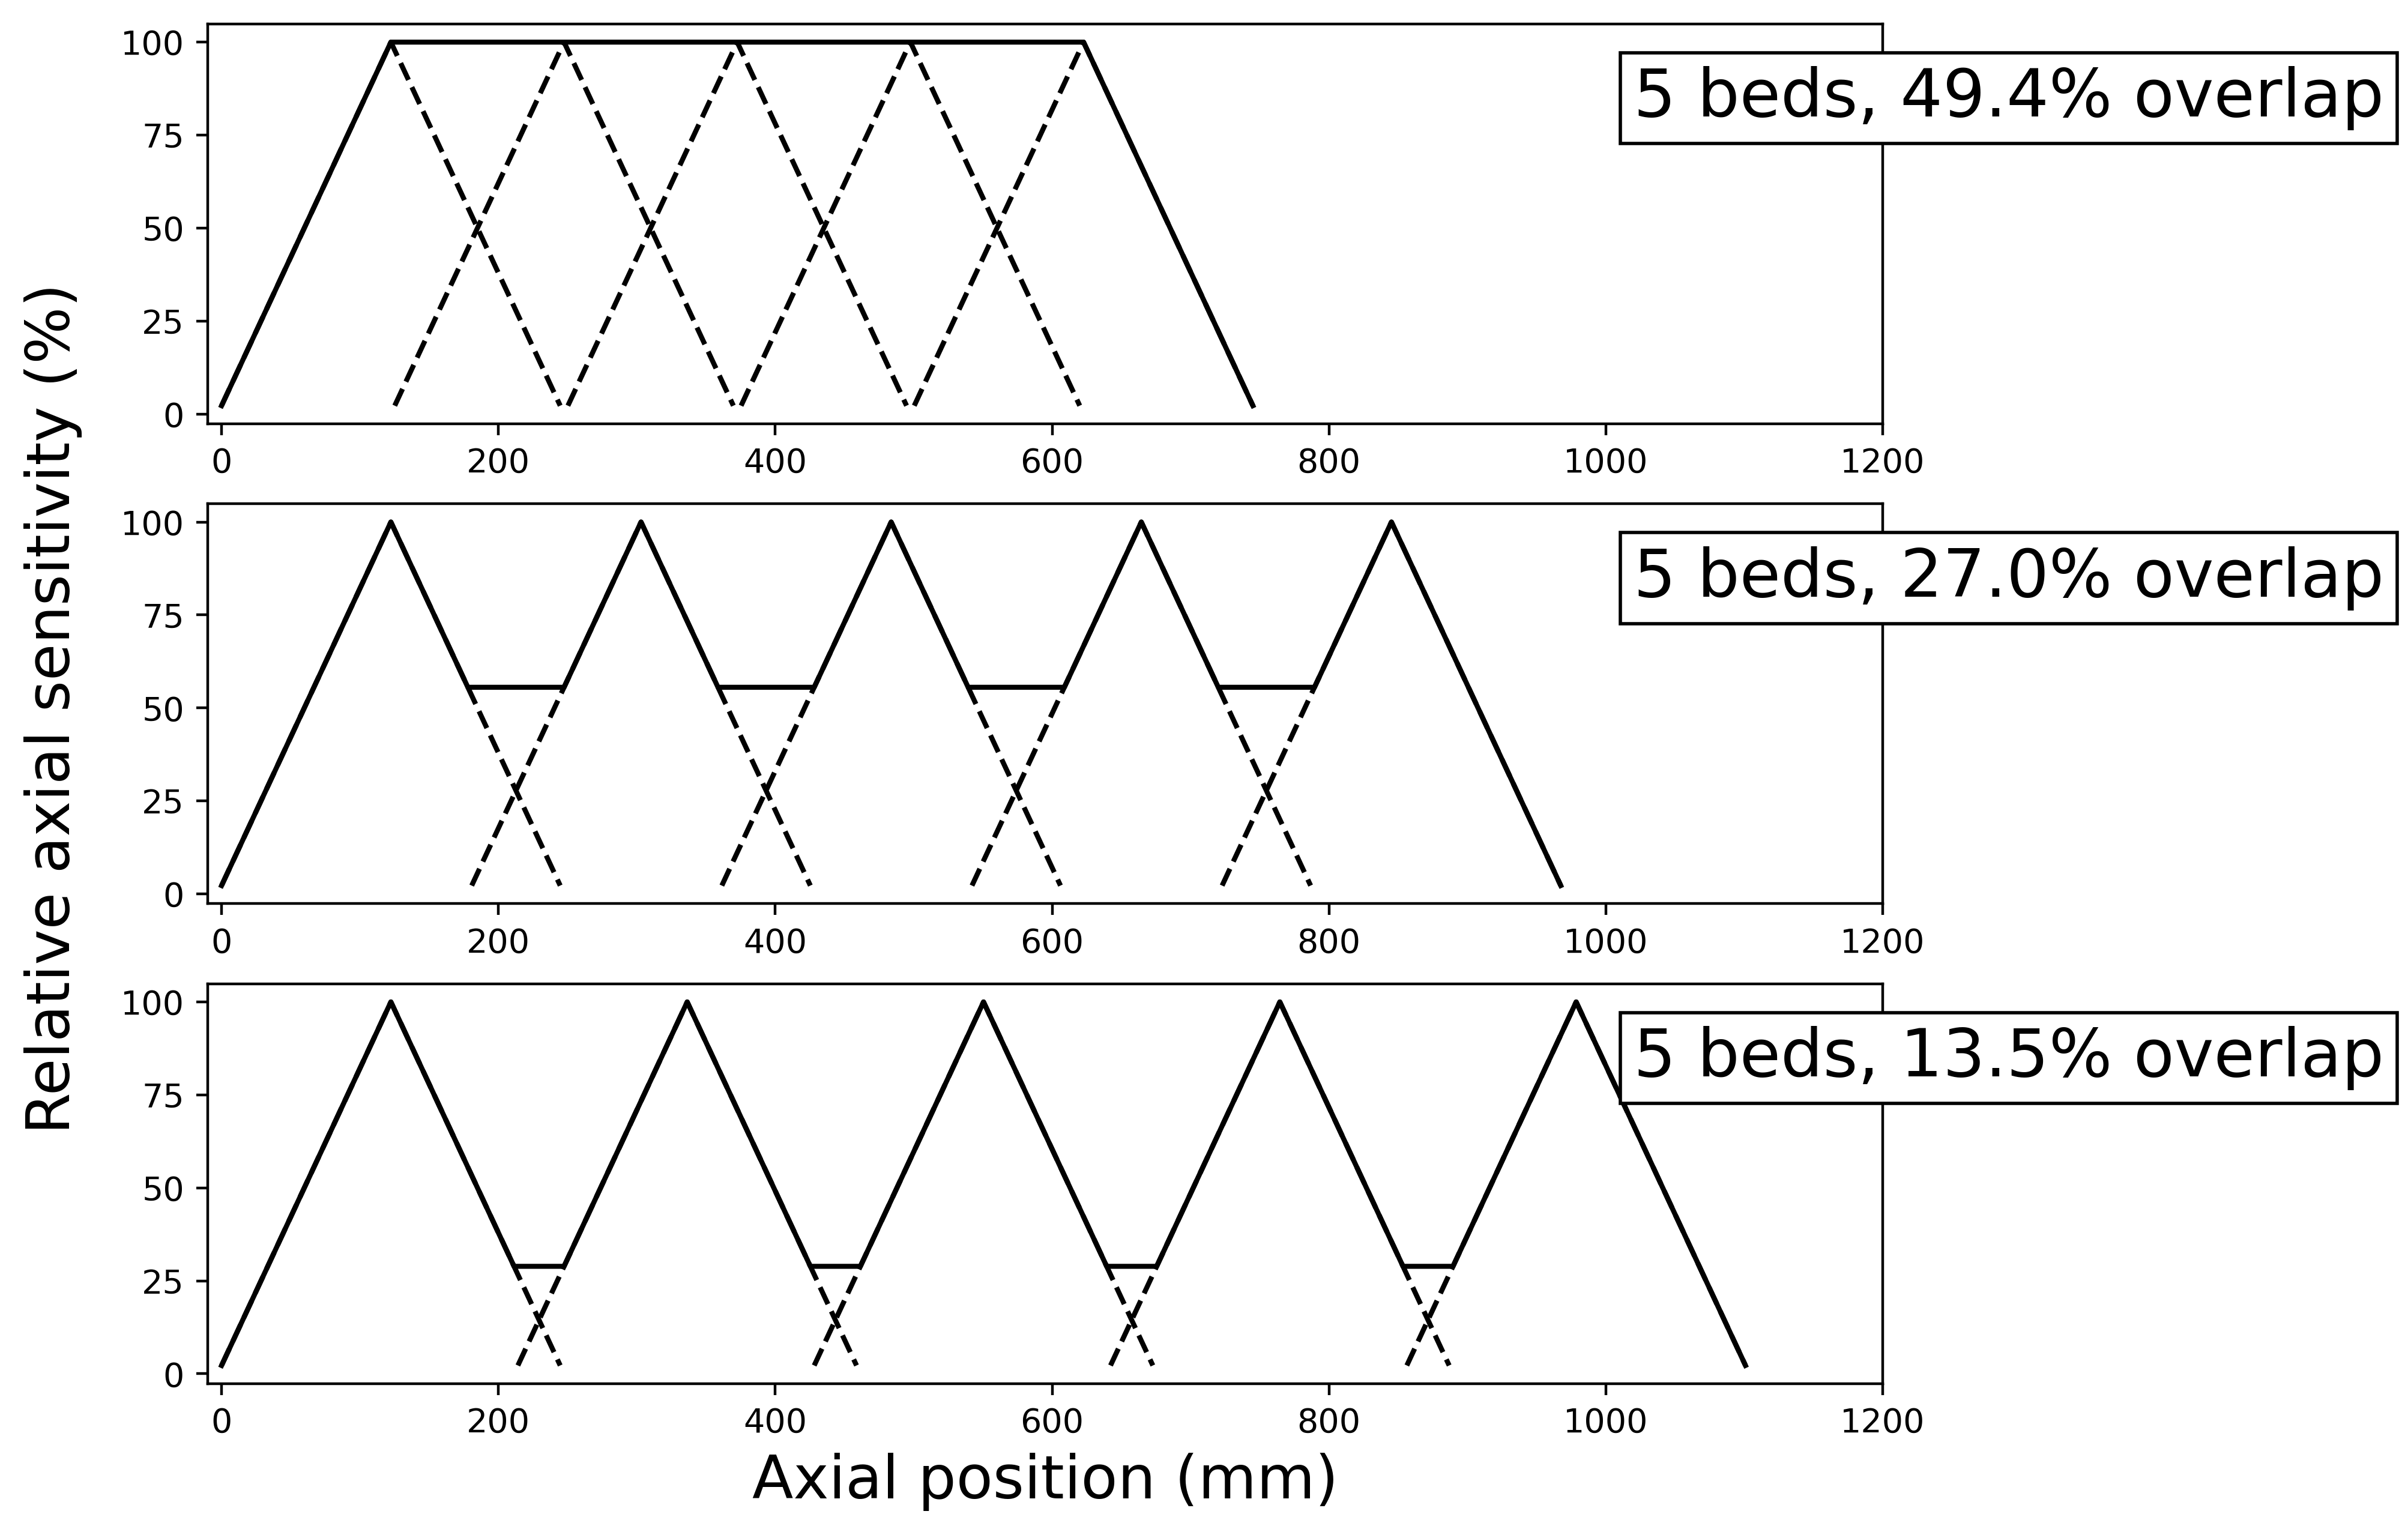
\includegraphics[scale=0.5,angle=0]{3_Results/3_1_DWB_Optimization/figures/SensitivityProfiles_3Options.png}
\caption{Relative axial sensitivity of 5 bed positions with decreasing overlap.} 
%TODO: Add over-scan in the CBM D-WB protocols. 
\label{fig3_1:decreasingOverlap}
\end{figure}
%
%
\begin{figure} [ht!]
\centering
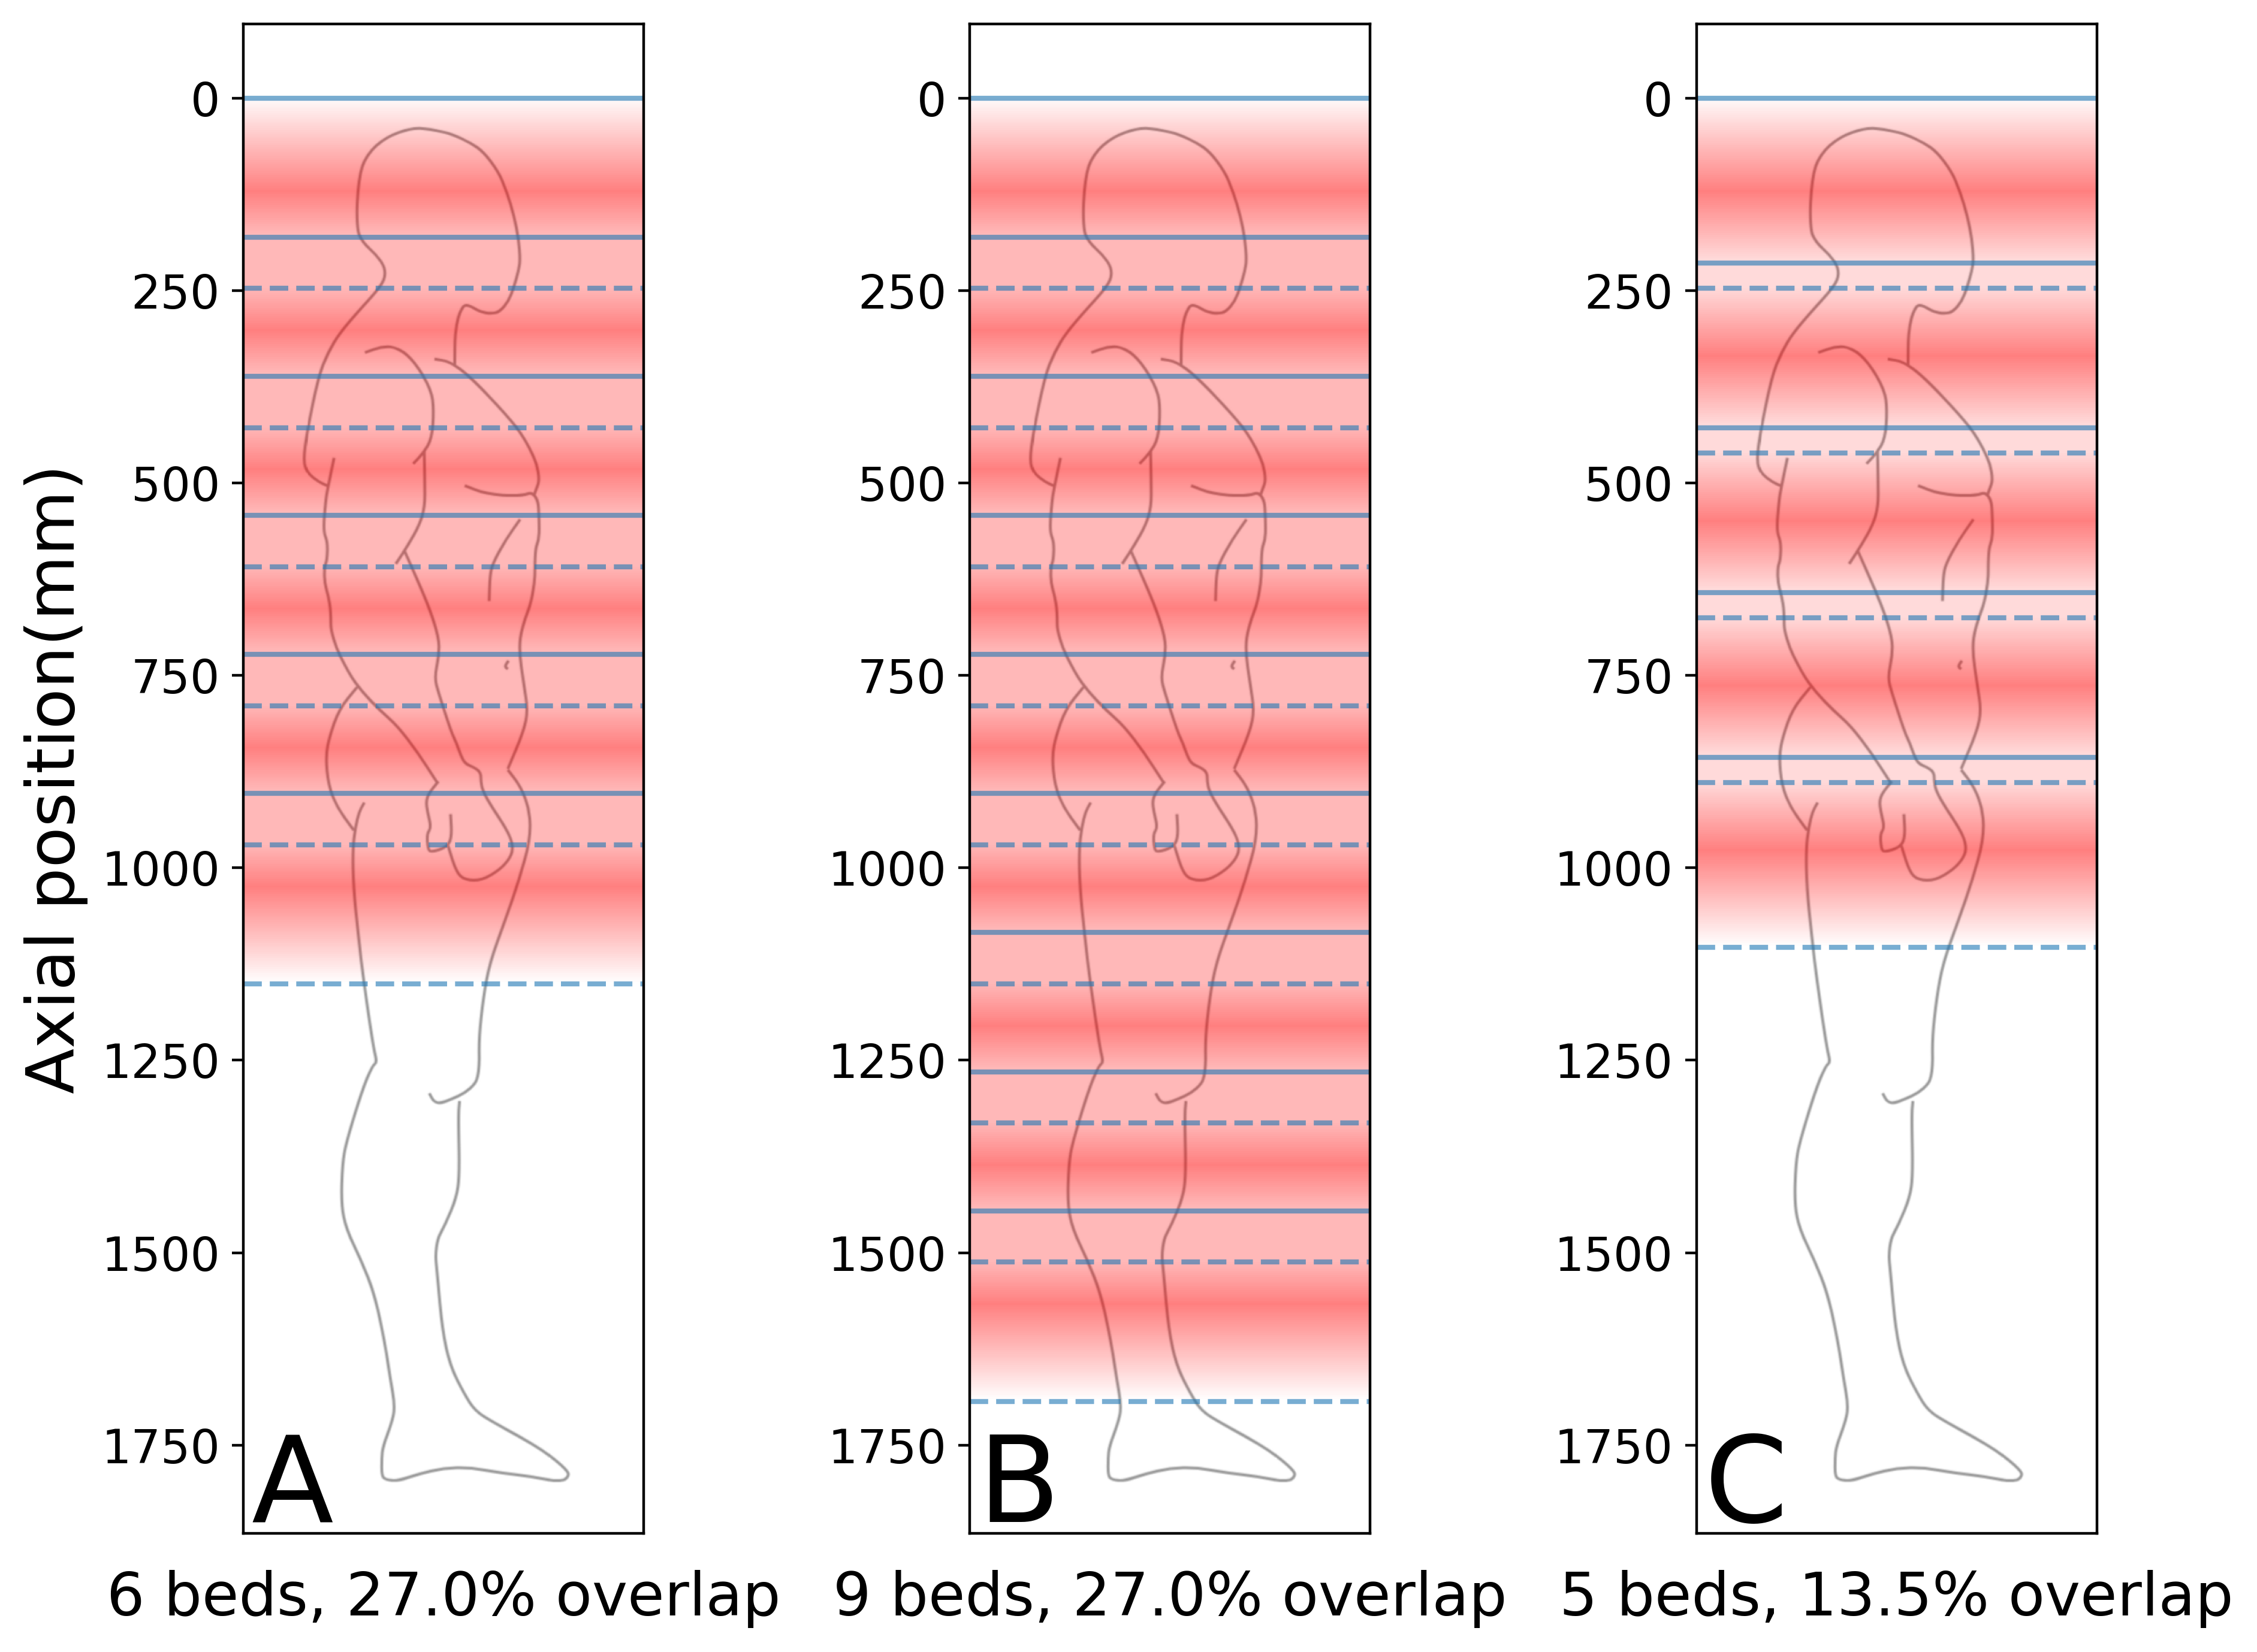
\includegraphics[scale=0.5,angle=0]{3_Results/3_1_DWB_Optimization/figures/SensitivityProfiles_overHuman.png}
\caption{Combinations of overlap and number of beds for static (A\&B) and dynamic whole-body imaging(C). Relative axial sensitivity is shown in shades of red, with bed start (\protect\tikz[baseline]{\protect\draw[line width=0.5mm] (0,.8ex)--++(1,0) ;}) and end (\protect\tikz[baseline]{\protect\draw[line width=0.5mm,densely dashed] (0,.8ex)--++(1,0) ;}) positions.} 
%TODO: Add over-scan in the CBM D-WB protocols. 
\label{fig3_1:BodyCoverage}
\end{figure}



\subsection{Continuous Bed Motion}
Continuous Bed Motion was proposed as an extension of step and shoot acquisition performed with small steps, to provide uniform axial sensitivity profiles without the need of overlaps~\cite{Dahlbom2001,Brasse2002}. In clinical CBM acquisition protocols prompt data as well as bed positions information are stored in list-mode during the examination, with the data being sorted after or during the examination in sinograms (refereed as "chuncks") before reconstruction. The velocity of the bed movement can be adjusted depending on the amount of desired collected statistics, similar to the acquisition time per bed in step and shoot acquisitions. With recent systems the bed velocity can also be varied within an examination according to the needs and distribution of the imaged activity~\cite{Panin2014}. Beyond the potential technical gains, CBM protocols have also been shown to aid in patient comfort during examination~\cite{Schatka2016}. 

In particular for dynamic whole-body imaging many aspects of CBM acquisition can be beneficial over SS imaging~\cite{Karakatsanis2016}.  

\section{Dynamic WB PET}
As outlined in the Introduction and Methods section, clinical and research applications can benefit from dynamic whole-body (DWB) PET information. In clinical applications DWB data can be used to construct fully quantitative parametric images for diagnosis and response monitoring of disease and pathology over the whole body. In research DWB information can enable studying of the whole body organism and interactions between different tissues, organs or compartments. 

Although recent advancements in PET have led to development of PET/CT systems with increased A-FOV, with approximately half~\cite{Karp2020,Siegel2020} or even total-body axial coverage~\cite{Cherry2018}, the majority of PET systems in use are limited in the range from 15 to 26 cm~\cite{Vandenberghe2020}. 
Based on the same principles and methods used in static WB PET imaging, DWB protocols have been developed with use of repeating whole-body passes (often refereed as "sweeps"). These can be implemented as SS protocols, as proposed in the original work on multi-bed DWB protocols by Karakatsanis ~\textit{et al.}~\cite{Karakatsanis2011,Karakatsanis2013}, or as later proposed using CBM~\cite{Karakatsanis2016,Hu2020}. Such protocols are nowadays implemented in commercial PET/CT systems~\cite{Hu2020} and it has been shown that their use in clinical practice is feasible~\cite{Fahrni2019,Dias2020}.  Their usefulness in clinical imaging over static imaging practices is an ongoing active area of research and yet to be proven. 

\subsection{Challenges in multi-bed DWB protocols}
DWB studies, similarly to single-bed single-organ dynamic studies, are limited to a total duration of one hour, for practical and patient comfort reasons. 
But the transition from single-bed to multi-bed acquisition poses some limitations. 
The immediate effect of transition from single bed dynamic studies to multi-bed dynamic studies is the introduction of temporal gaps in the acquired data of any given bed position. These are introduced at each bed position by the time spent on imaging other bed positions and by scanner system delays caused by time taken for bed movements and by the system electronics to prepare for each acquisition. These gaps cause a significant reduction in the sensitivity of the acquisition, with fewer total counts collected for each axial location when compared to single bed dynamic acquisitions. Furthermore, estimation of fast temporal changes in tracer uptake are compromised as the early time points of the acquisition are not fully sampled for all beds. Finally clinical protocols further sacrifice scan time, for accommodating image derived input function (IDIF) estimations which are required for maintaining a non-invasive examination. These are made using an initial single bed dynamic acquisition, centred over the heart and the aorta, for a duration of a few minutes before commencing the DWB multi-bed acquisition~\cite{Karakatsanis2013,Hu2020}.
For research applications, particularly using new tracers which require metabolite analysis, the input function is frequently measured with invasive measurements via an arterial catheter. In these cases the use of the initial single-bed dynamic (SBD) phase is optional. But when estimation of pharmacokinetic parameters of interest that require full sampling of the early kinetics is needed, the single-bed dynamic phase can be included to estimate those parameters over a region of interest covered by the single-bed AFOV. Such use of the single-bed dynamic phase in clinical studies has also been recently explored for estimation of micro-parameters and their potential clinical applications~\cite{Zaker2020}.

Without previous knowledge, normally equal weight is given to the whole effective AFOV and so all bed positions are sampled equally with the same number of frames and so the number of WB sweeps within the DWB examination will depend on the number of frames per bed and vise versa. The number of frames that can be fitted within the study duration is limited by the system delay times, during which no data are acquired. As the characteristics of the system delays will vary for different imaging systems, it is expected that the framing will have to be adjusted for different systems too. Furthermore the expectation of the underlying kinetics, the expected tracer distribution and also the injected activity and half-life of the used radioisotope are factors that will have to be taken under consideration when considering the DWB protocol framing. 
An optimization methodology for such parameters is outlined by Karakatsanis \textit{et al.}~\cite{Karakatsanis2013}, used in their work conducted for the characteristics of the GE Discovery RX PET/CT scanner for FDG and Patlak imaging. 



\subsection{Latest technological advancements on long FOV PET systems}
Longer axial coverage was always a desirable characteristic for PET, but limitations in technology and costs only made it possible only during the recent years. Longer A-FOV scanners, with 70cm and 194cm length have been developed within the Explorer project in collaboration with United Imaging~\cite{Cherry2017,Badawi2019}. A 106cm long PET-CT scanner is also now commercially available by Siemens~\cite{Siegel2020}.  The models that are able to encompass the entire body at once, are referred as total-body systems. 
The increase of axial length offers many potential benefits for clinical and research applications. Most of those are linked to the increase in sensitivity offered by the greater A-FOV and number of total detectors. From 20cm to 100cm A-FOV an sensitivity increase of 2-3x is expected for single organ studies, but that is increased to 10-20x for whole body examinations~\cite{Vandenberghe2020}. The increased sensitivity can be used for performing ultra short or ultra low dose imaging, or a combination of both. This type of technology also offers the opportunity for whole-body dynamic imaging in clinical and research applications. 
